\documentclass[crop=false,class=mitthesis,oneside,font=12pt]{standalone}
%----------------------------Preamble-------------------------------%
\usepackage{amsmath}
%\newcommand{\angstrom}{\textup{\AA}}
\usepackage{microtype}
\usepackage{graphicx}
\graphicspath{{./images/}}
%\usepackage{multirow}
\usepackage{rotating}
\usepackage{natbib}
\usepackage{url}
\usepackage{booktabs}
\usepackage{makecell}
\usepackage{graphicx, float}            % Graphics/Images.
\usepackage{pgfplots, tikz}             % Drawing/graphing tools.
\usetikzlibrary{
    calc,                   % Calculating right angles and more.
    angles,                 % Drawing angles within triangles.
    arrows.meta,            % Latex and Stealth arrows.
    quotes,                 % Adding labels to angles.
    positioning,            % Relative positioning of nodes.
    decorations.markings,   % Adding arrows in the middle of a line.
    patterns,
    arrows,
    shapes,
    shapes.geometric,
    cd,
    hobby,
    babel
}                                       % Libraries for tikz.
\pgfplotsset{compat=1.9}                % Version of pgfplots.
\usepackage[]{pdfpages}
% for line numbers comment the next two lines before final submission
\usepackage{lineno}
\linenumbers*[1]
% use fancyhdr, to enable page style stuff (below)
\usepackage{fancyhdr}
\setlength{\headheight}{15.2pt}
\renewcommand{\headrulewidth}{0pt}

\pagestyle{plain}
\usepackage{import}                     % Import external files.
\usepackage[subpreambles=false]{standalone}      % Complileable sub files.
\begin{document}
\chapter{Was the total solar eclipse of August 21, 2017 responsible for the Traveling Ionospheric Disturbances observed in airglow observations ?}
In this chapter, background on Atmospheric Gravity Waves (AGWs) and associated Traveling Ionospheric Disturbances (TIDs) observed via airglow perturbation measurement is provided. Specifically, the possibility of the total solar eclipse of August 21, 2017 causing the AGWs that were observed by HiT\&MIS's airglow measurement eight hours after the eclipse had passed is discussed. 
\section{Background} 

Atmospheric Gravity Waves (AGWs) manifest as Traveling Ionospheric Disturbances (TIDs) via ion-neutral coupling in the Ionosphere-Thermosphere (IT) system \citep{hines_1960}. TIDs are wave-like plasma oscillations in the ionosphere that can be triggered by various processes (including AGWs) and occur at different temporal and spatial scales. TIDs with wavelengths of 100--300~km are classified as Medium Scale TIDs (MSTIDs) and can be caused by various processes, but in general are associated with tropospheric forcing \citep{kelley}. TIDs with wavelengths larger than 1000 km and with time periods greater than one hour are classified as Large Scale TIDs (LSTIDs) \citep{hocke1996review}.

Most LSTIDs propagate from either pole and are associated with magnetic disturbances. Geomagnetic storms cause rapid enhancement of the auroral electrojet (related to the Hall current) that leads to thermospheric heating and expansion \citep{davis_polar_1971,chimonas_atmospheric_1970}. This generates AGWs that propagate toward the equator. The divergence of AGWs in turn generates LSTIDs \citep{prolss_lstid_2000}. LSTIDs that have propagated equatorward and are associated with geomagnetic storms have been observed by previous studies (see \citet{habarulema_storm_tid}, and references therein). For example, based on magnetometer measurements, \citet{habarulema_storm_tid} showed that equatorward TIDs were launched following a southward turning of the Interplanetary Magnetic Field (IMF).

Besides geomagnetic storms, solar eclipses are also known to excite AGWs \citep[e.g.,][]{liu_1998, chimonas1970}, that alter the  IT system~\citep{Lin2018,harding_nightside_eclipse}. \citet{liu_1998} conclude that the ionospheric perturbations that they observed using ionosondes during the total solar eclipse of October 24, 1995 was most likely due to plasma up-flow and down-flow resulting from the cooling and decrease in photo-electron production induced by the eclipse.

\citet{coster_gnss_2017} found signatures of possible mountain waves, using Total Electron Content (TEC) maps, during the August 21, 2017 eclipse. Furthermore, for the same eclipse event, \citet{goncharenko_mh_hill_eclipse} used co-located measurements of digisonde and the Millstone Hill ISR (Westford, MA, $\sim$ 60\% peak obscuration), and observed a fast (20-40~m/s) upward plasma drift above the peak height of the F2 layer, hmF2, immediately following the maximum obscuration. Neutral wind velocity derived from night-time OI 630.0~nm (red line) emission measurements by a Fabry-Perot Interferometer (FPI) in Brazil showed perturbations in neutral winds far from the path of the August 21, 2017 eclipse. Global-scale simulations using a UV obscuration mask that mimicked the August 21, 2017 eclipse's effect on the upper atmosphere successfully predicted the measured changes (using the red line) in neutral wind qualitatively \citep{harding_nightside_eclipse}.

% The 2017 solar eclipse occurred over the continental USA where numerous satellite receiver and ground based instruments were present, leading to abundance of data for studying the effects on the upper atmosphere. Some of the studies have already resulted in observation of unexpected phenomenon. \citet{coster_gnss_2017}, based on Total Electron Content (TEC) measurements, saw enhanced TEC structure along the Rocky mountains as the eclipse passed through them. Based on differential TEC (dTEC) measurement and EUV occultation map, \citet{mrak_eclipse_2018}, found that the large-scale perturbation structure in dTEC immediately following the eclipse mimicked the gradient of the EUV map. This led them to theorize that the perturbation seen in TEC was a directly a consequence of EUV modulation during the eclipse not AGW's.

On August 22, 2017 a sequence of LSTIDs was observed in the northern hemisphere, following a minor geomagnetic storm (minimum Dst index $\sim$-30 nT, peak Auroral Electrojet index $\sim$1000 nT) over North America. The geomagnetic storm followed the eclipse of August 21, 2017 that occurred 8 hours earlier at Carbondale, IL. In this chapter, first, a comprehensive LSTID analysis is presented by virtue of simultaneous measurements by: ground-based spectral imager, Global Positioning System (GPS) differential TEC maps, and ionospheric parameters derived from digisonde. Then, the TID event analysis and characterizing of the TID wave parameters are discussed in detail. The dominant time period in all of these measurements was found to be around 1.5 hours. In addition, the observations are compared to simulations with the Global Ionosphere-Thermosphere Model (GITM) \citep{ridley_global_2006} to ans if the observed TIDs were generated due to the effect of the eclipse.

\section{Measurements}

\subsection{Spectral measurements}

The TIDs were observed from Carbondale, IL (Geographic location: 37.7$^\circ$N, 89.2$^\circ$W) using the High Throughput and Multi-slit Imaging Spectrograph (HiT\&MIS) \citep{hitmis}. HiT\&MIS can simultaneously measure six upper atmospheric emission features at high resolution ($\sim$ 0.02~nm/px in red line, for example). The field-of-view (FOV) of HiT\&MIS is approximately 0.1$^\circ$ by 50$^\circ$ and was centered at an elevation angle of 45$^\circ$ looking towards the northwest (Figure \ref{fig:elayer}). The spectral images were recorded at a cadence of 4 minutes using a CCD camera from 2--10~UTC on August 21 and 22, 2017. Simultaneous measurements in the red line and green lines are used for this particular study. 

\begin{figure}[H]
	\centering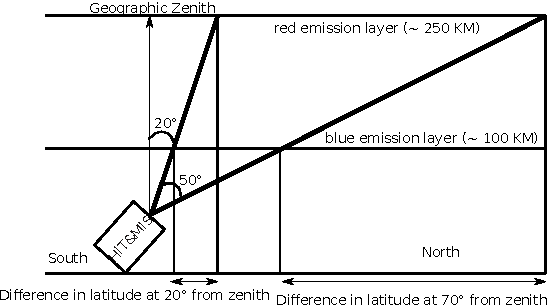
\includegraphics[width=30pc]{elayer.pdf}
	\caption{Viewing geometry of the HiT\&MIS instrument August 21-22, 2017 at Carbondale,IL. The latitudes traced by the red and green lines are shown assuming the peak emission height of 250 km and 123 km, respectively. Note that for line of sites closer to the zenith (higher elevation angles), the range of latitudes covered by each emission layer is smaller. However for line of sights closer to the horizon (lower elevation angles), emission from a larger latitude range are integrated along the line of sight.}
	\label{fig:elayer}
\end{figure}

From the raw CCD images, wavelength regions around the red and green lines, plus a diagnostic cloud indicator also observed by HiT\&MIS, were extracted as a function of HiT\&MIS elevation angle and wavelength.  The NeI 630.5 nm line (present in street lights) was used as an indicator of cloud activity as reflection of street lights from clouds acts as a proxy for sky conditions. See Chapter 2 for a more detailed description of the spectra extraction procedure for HiT\&MIS.

For each feature at each time-stamp, the brightness is obtained by co-adding signals from all wavelength bins around $\pm$0.3 nm from the line center. The brightness is then plotted as a function of elevation angle and time. GLOW \citep{solomon_1988,solomon1989630,bailey2002} model estimates of the Volume Emission Rate (VER, not shown) provides the peak heights of the red (250~km) and green (150~km) lines in the thermosphere. In addition, the green line has another peak in the mesophere region (96~km \citep{yee1987}), the average of the thermospheric and the mesospheric peak heights is assumed to be the peak green line emission height (123~km). Using these emission heights and the viewing geometry of HiT\&MIS, the elevation angles are then converted to the latitude of the emission height projected on the ground. 

\subsection{GPS Differential TEC measurements}
\label{tec}
In order to compare the airglow brightness morphologies in the spectral data, the differential Total Electron Content (DTEC) maps were used. Continuously Operating Reference Stations (CORS, www.ngs.noaa.gov/CORS) and Crustal Dynamics Data Information System (CDDIS, cddis.nasa.gov) publicly available databases with Global Navigation Satellite Systems (GNSS) observation data were used to obtain the DTEC. This accounted for a total of  $\sim$1800 receivers in the continental US. 

To compute the phase-corrected slant TEC estimates, the approach of \cite{Coster1992} is used. The slant TEC were converted to the vertical TEC (vTEC) via a mapping function applied at 300~km altitude \citep{Klobuchar1987}. The background vTEC are then subtracted to obtain DTEC residuals, using variable orders of polynomials \citep{Mrak2018}. The carrier phase based differential approach provides better accuracy up to 0.03~TECu \citep{Coster2012} (1~TECu = 10$^{16}$e$^-$/m$^2$). The DTEC residuals were mapped to a geographical map at an altitude of 300~km and transformed from the naturally irregular spatial grid into a regular grid \citep[e.g.,][]{Azeem2015, Mrak2018} with a resolution of 0.2$^\circ$ $\times$ 0.2$^\circ$ (geographical coordinates). The differential approach and large spatial coverage ($\sim$15,000 spatial data points at a given time) allow one to extract coherent spatial features of tiny amplitudes. The spatial extent and appearance of the coherent perturbations are presented in the form of 2D projections. The DTEC time series observations for locations aligned with the HiT\&MIS FOV are also obtained. 

\subsection{Digisonde measurements}
\label{digi_m}

An additional insight into the nature of observed TIDs is provided by the Global Ionosphere Radio Observatory (GIRO) \cite{reinisch2011global}, a network of \textit{ionosondes}, high-frequency (HF) bottomside ionosphere sounders. Two GIRO locations operated by Idaho National Laboratory at Idaho Falls, ID (INL, 43.5$^\circ$N, 112$^\circ$W) and by University of Massachusetts Lowell at MIT Haystack Observatory, Millstone Hill (MH, 42.5$^\circ$N, 71.4$^\circ$W) were selected. Both observatories employed the latest Digisonde model DPS4D \citep{reinisch2009new,digisonde.com} in its high-cadence campaign mode, recording the vertical sounding ionograms once a minute. 
% * <temujinparuhang@gmail.com> 2018-10-29T18:26:28.356Z:
% 
% > \citep{reinisch2009new,digisonde.com
% Doest show up as a clickable link. Not sure if it will in the published form
% 
% ^.

Since the first report of the TID phenomenon detected by means of HF radio interferometry \citep{munro1950travelling}, ionosondes have been used as reliable TID detectors with well-established sensitivity to plasma perturbations, as even minute changes of the electron density cause easily detectable variability of the signal propagation path in the ionosphere. For the current investigation, time series of the Maximum Usable Frequency (MUF) at a distance of 3000 km (D), MUF(D)F2, a standard ionogram-derived characteristic is used. MUF(D)F2 (referred to as MUF hereafter) is obtained numerically using the shape of the O-wave signal trace extracted from the ionogram (see \cite{davies1989ionospheric} for details) and its change reflects variability in both peak density and height of the F2 layer. This thus enhances the overall sensitivity to plasma perturbations in comparison to individual analysis of the ionospheric characteristics describing density, reflection height, or columnar content of the ionosphere.

\section{Results}

\subsection{Spectral Data}
 The red and green line brightnesses for the night of the eclipse and TID event (August 22, 2017) are presented in Figure \ref{fig:keo_profile}. The brightness data for the night before the eclipse (August 21, 2017) are also shown for comparison. The red and green line brightnesses on the night with the TID event (August 22) show wave-like brightness perturbations, while the perturbations on the night before (August 21) only coincide with the cloud-indicator, especially in the green line.

\begin{figure}[H]
 \centering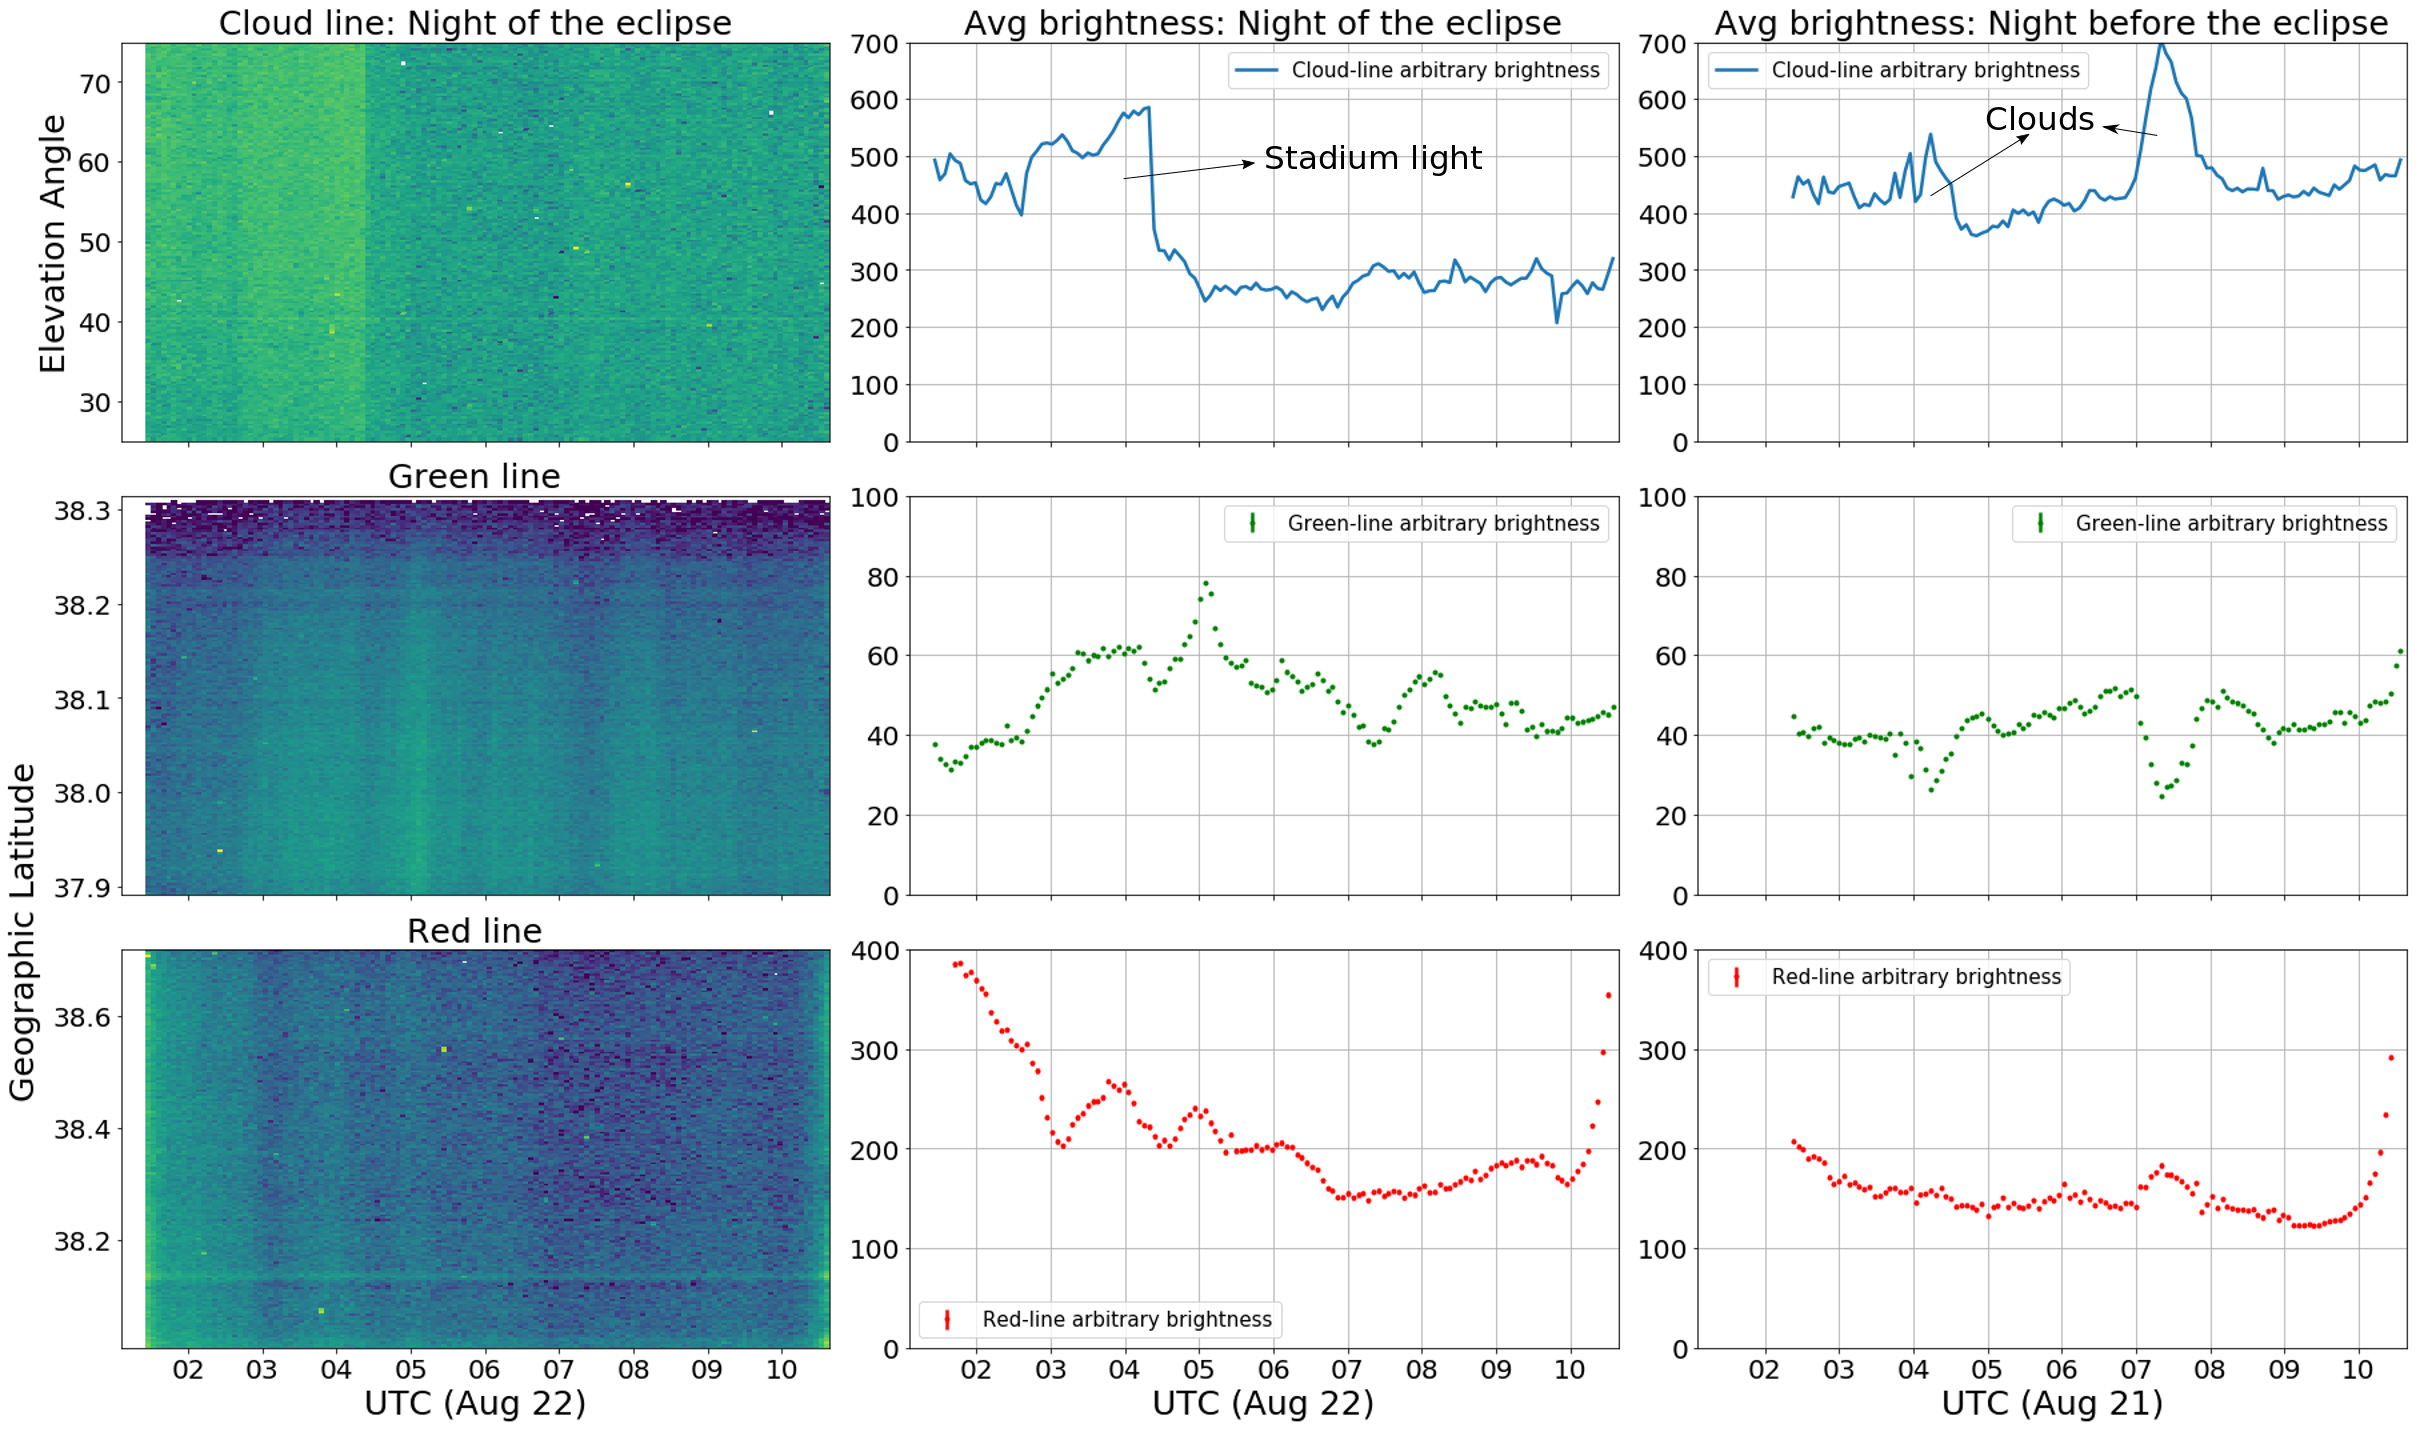
\includegraphics[width=35pc]{car_Aug2122_both.png}
 \caption{Left column: Brightness keogram of Ne I (cloud indicator, top), green line (middle) and red line (bottom) as a function of look direction (or latitude) on the night of the eclipse (Aug 22). Brighter color represents higher brightness (in arbitrary units).  
 %White-space represents negative values encountered after baseline subtraction. 
Center column: Brightness averaged over the whole field of view (0.1$^\circ$ by 50$^\circ$) for each representative keogram on the left. Notice clear wave-like perturbations seen in both red and green lines on August 22. Right column:  Same as the center panel but on the night before the eclipse (August 21, keogram not shown). The dips in the green line coincides with the increase in the cloud line brightness. There is a sudden drop in the cloud-indicator brightness around 4~UTC on August 22, this is due to nearby stadium light, which was in HiT\&MIS FOV, being switched off. This is not seen in the red line possibly because the wings of the NeI 630.5 nm spectra leaked into the red line (630.0 nm).  The cloud-indicator level on August 22 are around the same level as August 21 even with the stadium light leak, and lower after the stadium light was turned off. }
\label{fig:keo_profile}
\end{figure}

\subsection{DTEC data}
\begin{figure}[htp]
\centering
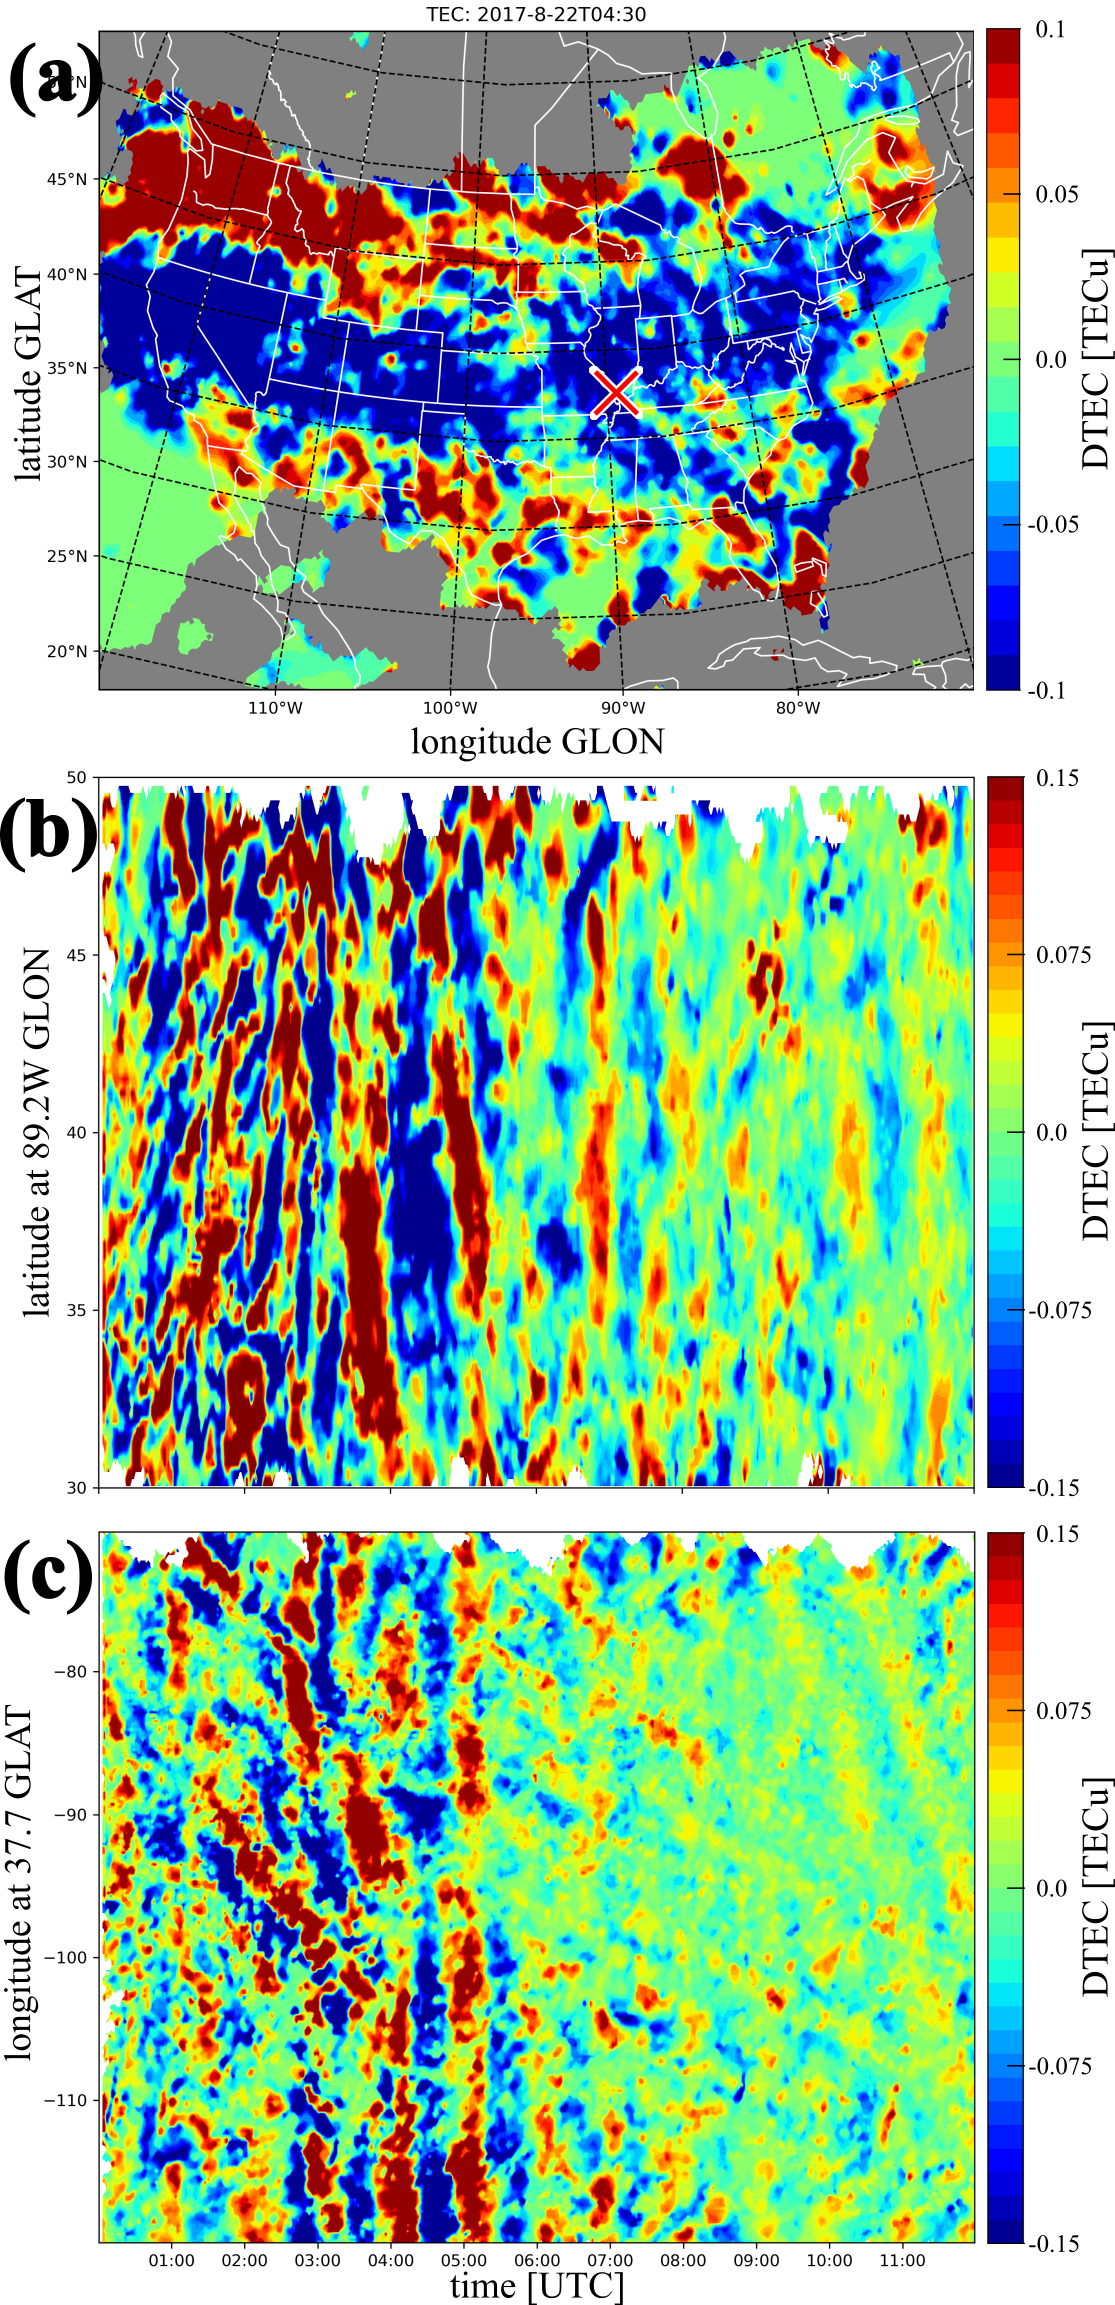
\includegraphics[width=23pc]{tec_map.png}
\caption{The LSTIDs event as observed by GPS-aided DTEC maps. (a, top) A representative GPS map of TIDs over continental US, at 4:30~UTC. Red 'X' mark denote the location of the HiT\&MIS instrument at Carbondale, Il (37.7$^\circ$N, 89.2$^\circ$W ) . (b, middle) A DTEC keogram elongated along 89.2$^\circ$W longitude. (c, bottom) A DTEC keogram elongated along 37.7$^\circ$N latitude.}
\label{fig:tecmap}
\end{figure}

To validate the wave-like brightness perturbation seen in the spectral data, DTEC maps over the continental USA were used. Figure~\ref{fig:tecmap} shows an example of the GPS-derived DTEC maps and a set of keograms crossing the location of the HiT\&MIS instrument. Figure~\ref{fig:tecmap} (a, top) shows the geographical extent of the large-scale perturbations at 4:30~UTC, when the geomagnetic activity was already in the recovery phase. The LSTIDs are compact and uniform in longitudes west from $\sim$100$^\circ$, whereas eastward they have latitudinal structures. This is an approximate line of geomagnetic declination angle 0$^\circ$ that the structures could be associated with. Further, keograms in Figure~\ref{fig:tecmap}b-c show the temporal extent of the LSTIDs in meridional and zonal direction above the HIT\&MIS location. The peak TID activity was observed in the time range between 3 -- 6~UT. Figure \ref{fig:dtec_carb} shows concurrent, co-aligned time series of DTEC and the dynamic part of the red and green line profiles obtained by polynomial de-trending at Carbondale, IL. The perturbations in the DTEC and in the green and red line brightness coincide between 03--06~UTC, which is also the time period when significant large-scale perturbations were observed in the DTEC keogram (Figure \ref{fig:tecmap}). 

\begin{figure}[H]
	\centering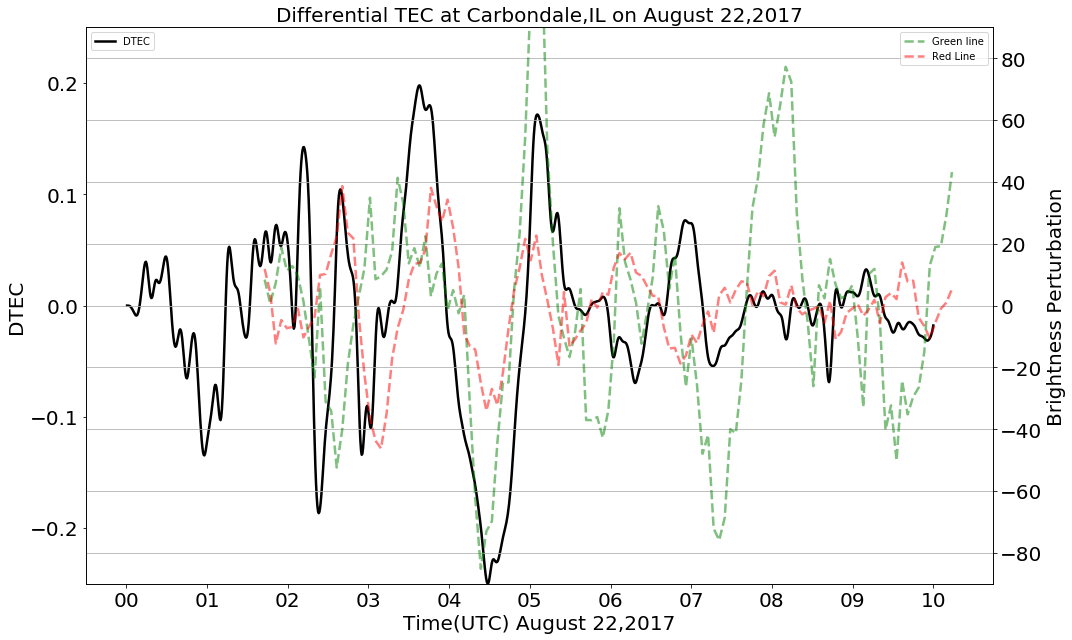
\includegraphics[width=35pc]{aug22_dtec_bper.png}
	\caption{DTEC obtained for Carbondale, IL on August 22, 2017 from GPS-derived TEC measurements (solid lines).  Notice stronger perturbations  and better coincidence from 3--6~UTC (compared to the whole profile) with red and the green line profiles shown in dot-dashed and dashed lines, respectively. This time-frame also coincides with the stronger large-scale DTEC perturbation (Figure \ref{fig:tecmap}) and peak enhancement and recovery of the AE index (Figure \ref{fig:gindx}).}
	\label{fig:dtec_carb}
\end{figure}

\subsection{Digisonde MUF data}
GPS TEC measurements suggested large scale nature of the observed plasma waves. To study this further, the digisonde measurements of various ionospheric parameters from far away locations, Millstone Hill (MH) and Idhao National Lab (INL) were looked into. The profiles of foF1, foF2, and MUF are shown in Figure \ref{fig:digi_w} and shows that while the foF1 frequency drops sharp during the time of the eclipse, no clear perturbation structures can be seen. Furthermore, since the F1 layer disappears during the night no night-time foF1 measurements are available. This means no vertical nature of the observed LSTIDs could be studied using digisonde measurements in the current case. As discused in Section \ref{digi_m}, MUF is more sensitive to ionospheric perturbations so only MUF profiles are used for further analysis.
\begin{figure}[H]
\centering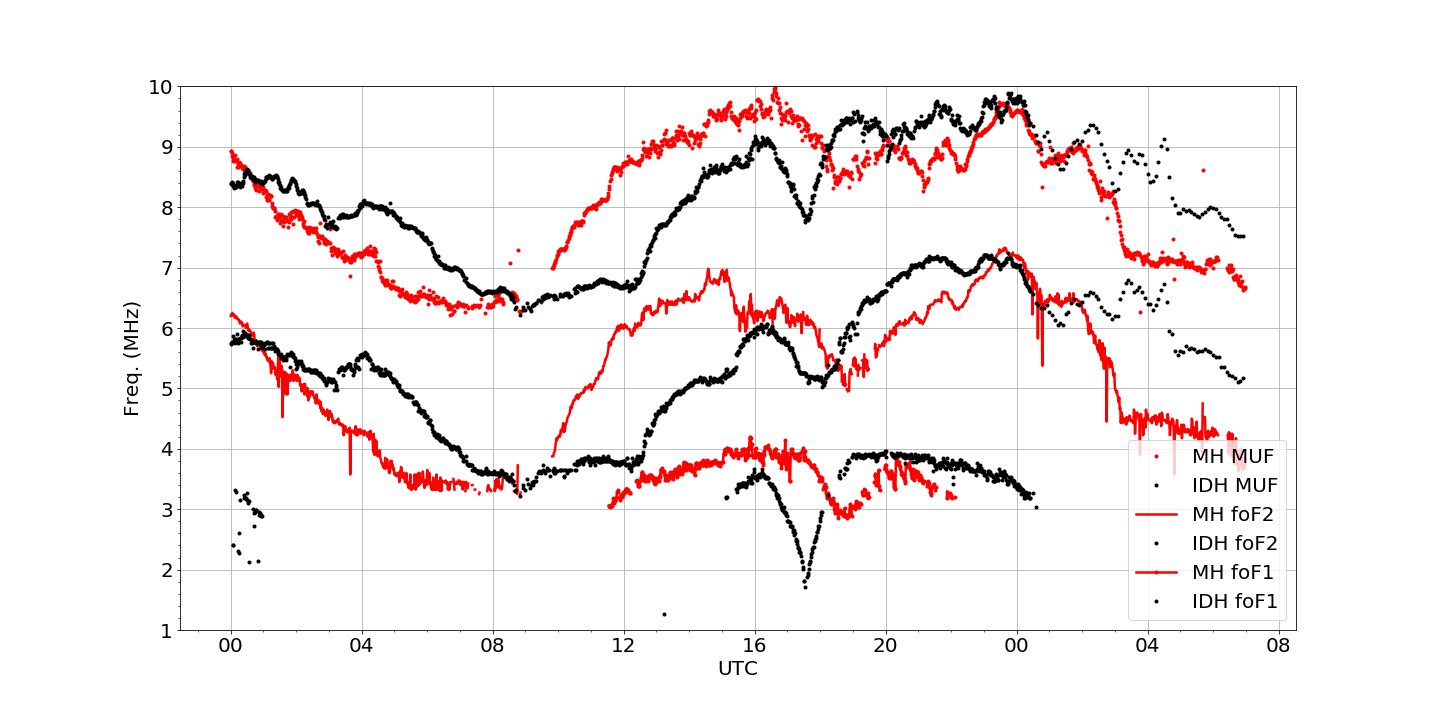
\includegraphics[width=35pc]{digi_21-22.png}
\caption{Digisonde-derived foF1, foF2 and MUF profiles at Idaho National Lab (INL) and Millstone Hill (MH)  on August 21 and August 22, 2017.}
\label{fig:digi_w}
\end{figure}

Figure \ref{fig:digi} shows the MUF timelines at MH and INL from 19~UTC on August 21, 2017 to 6~UTC August 22, 2017. The MUF variability is significant at both locations. The perturbations are also seen immediately prior to the start of geomagnetic disturbances (0~UTC on August 22, 2017). These pre-midnight perturbations might be associated with the after-effect of the eclipse, as \citet{goncharenko_mh_hill_eclipse} also reported enhanced plasma density over MH around 21~UTC (August 21) based on radar measurements, which they attributed to the eclipse's after effect. On the other hand, the post-midnight DTEC, brightness and MUF dynamics were more likely associated with the TIDs generated due to an increase in auroral currents as a result of enhanced geomagnetic activity. This is explained on the following section.

\begin{figure}[H]
\centering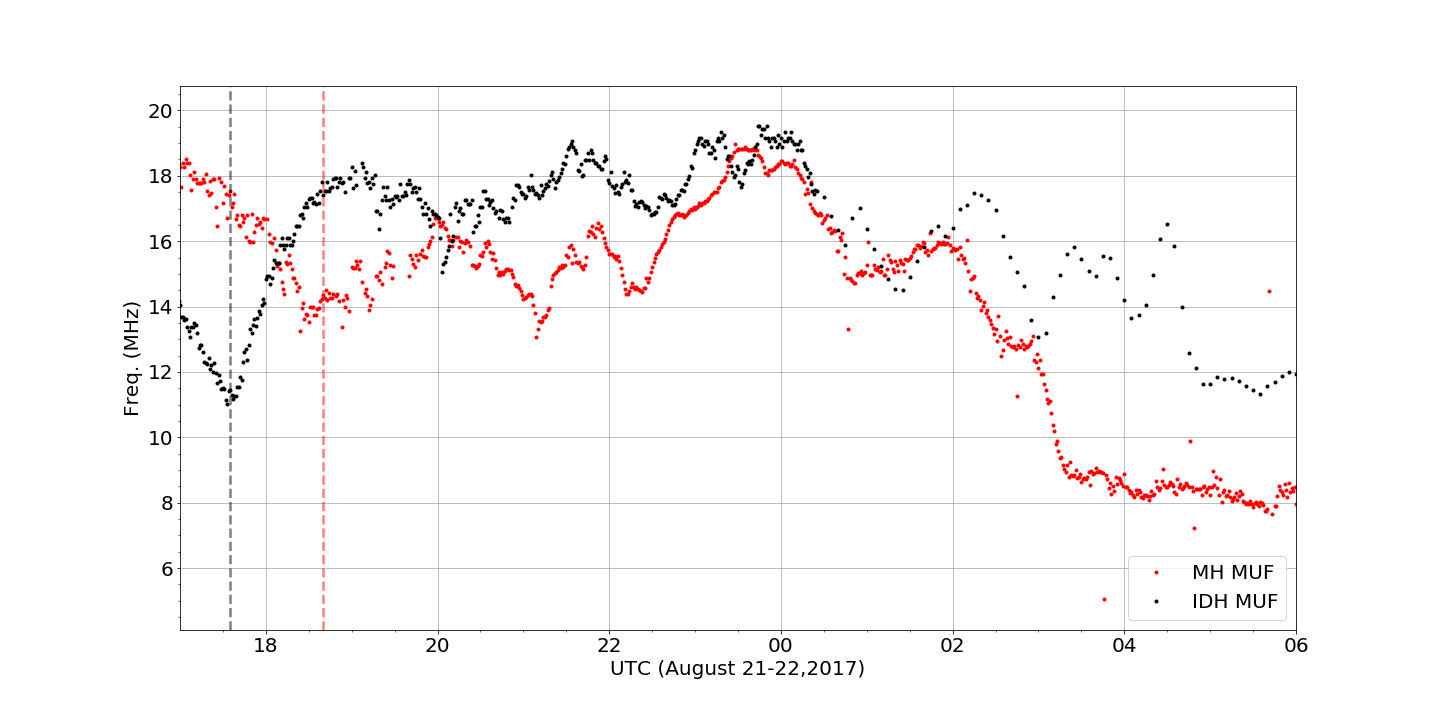
\includegraphics[width=35pc]{digi_muf_21-22.png}
\caption{Digisonde-derived MUF profiles at Idaho National Lab (INL) and Millstone Hill (MH) from 17~UTC August 21 to 6~UTC August 22, 2017. INL was close to the path of the totality and the  99\% peak obscuration time is shown by dashed-vertical black-line. MH was on the path of partial eclipse and the 60\% peak obscuration time is shown in dashed-vertical red-line. HiT\&MIS observation starts around 2~UTC on August 22.}
\label{fig:digi}
\end{figure}

\section{What caused the observed TIDs ?}
To understand the cause of the observed AGWs and TIDs, the geomagnetic conditions were analyzed. Figure \ref{fig:gindx} shows the Dst and the Auroral Electrojet (AE) indices from 18~UTC on August 21 to 10~UTC on August 22, 2017. The Dst  index is a measure of the equatorial ring current strength and is obtained by averaging ground-based measurements of magnetic fields near the equator. The AE index is a measure of the strength of auroral Hall currents and is obtained from magnetic field measurements near the polar cap. The AE strength is directly related to Joule heating of the IT system \citep{ae_joule} which, in turn, could potentially lead to equatorward propagating TIDs (see \citep{kauristie_dst} and references therein for details). 
  
LSTIDs arrived over the FOV at about 1~UTC and lasted until around 6~UTC. Likewise, the AE index began to intensify at approximately the same time, and relaxed back to prior values after 6~UTC. In addition, the keogram shows a complex structuring of the LSTIDs. The leading fronts initially arrived from the north-east and moved towards the south-west (1--4~UTC), but latter were almost perfectly elongated in the zonal direction (4--6~UTC). TIDs in smaller scales within the LSTIDs can also be observed; these are most likely caused wave breaking of the LSTIDs. It is thus concluded that the observed LSTIDs (and AGWs) were most likely generated by geomagnetic effects that induced changes in the auroral current leading to rapid heating and expansion of the thermosphere. Further insight is also gained by looking at the field aligned current measurements (Figure \ref{fig:fac}), which shows enhancement in FACs when compared to the night before.

\begin{figure}[H]
\centering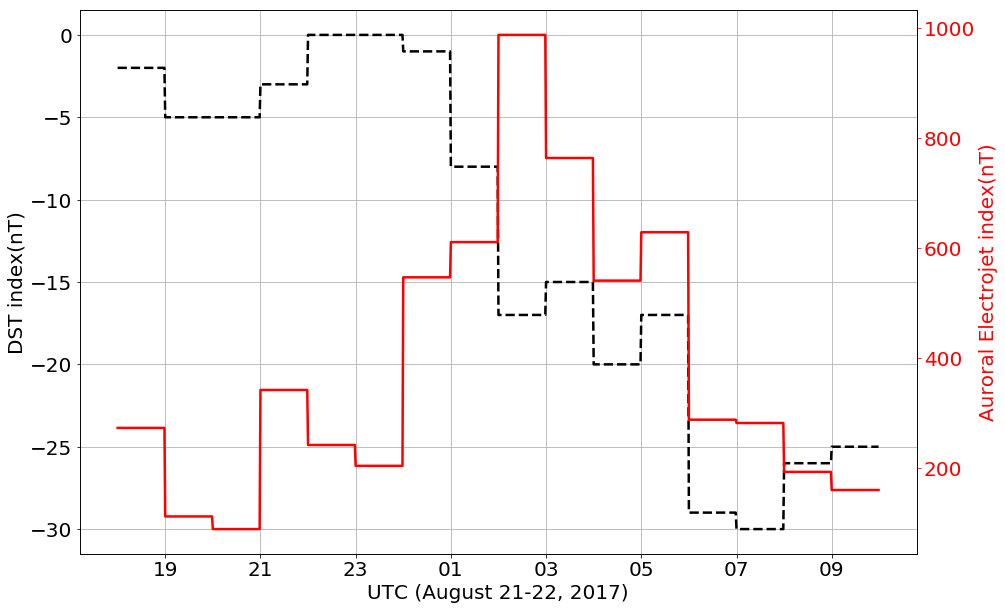
\includegraphics[width=30pc]{tid_geindex.png}
\caption{Dst and AE indices before and during HiT\&MIS observation times. Note the increase in AE starting at midnight UTC on August 22, 2017. }
\label{fig:gindx}
\end{figure}
\begin{figure}[htp]
\centering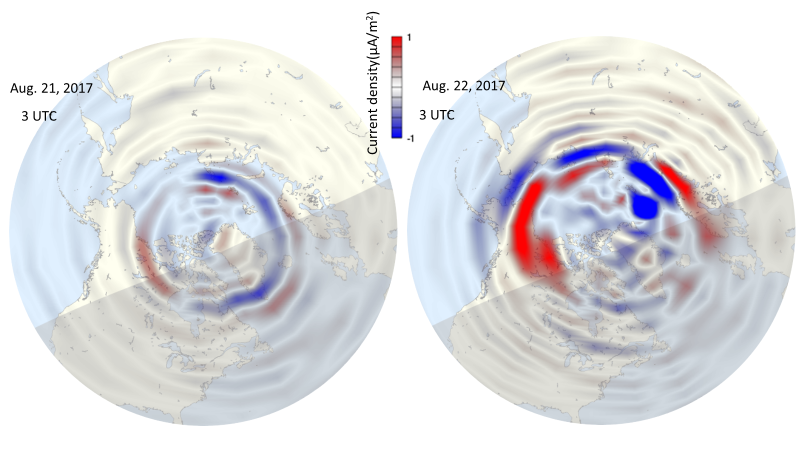
\includegraphics[width=35pc]{fac.png}
\caption{FAC at 3 UTC on August 21-22, 2017. Notice clear enhancement on August 22. }
\label{fig:fac}
\end{figure}

\section{Wave Characteristics}

Wavelet analyses is performed on the red and green line brightness profiles obtained at Carbondale, IL, digisonde MUF profiles obtained at INL and MH, and the DTEC measurements for Carbondale, IL. Wavelet analysis has been used by previous studies to identify wave characteristics of AGWs and TIDs \citep[e.g.,][]{singh_effect_2016,wvlt_B}. \citet{singh_effect_2016} studied the vertical propagation of AGWs due to a cyclone by performing wavelet analysis on optical emission brightnesses originating at different altitudes. \citet{wvlt_B} used wavelet analysis to study the variation in the geomagnetic field induced by eclipses.
 
The wavelet analysis is based on the guide presented in \citet{torrence_wavelet} and implemented using the Waipy package on Python (\url{https://github.com/mabelcalim/waipy}). Red and green line brightness profiles averaged over the whole FOV were used as there was no significant change in dynamic behavior as a function of elevation angle or latitude (see Figure \ref{fig:keo_profile}). 
The average brightnesses and MUF profiles were subtracted with a polynomial fit in order to remove the long-term climatological trends. The extraction of the dynamic part of the TEC measurement, DTEC, has been described in Section \ref{tec}. These dynamic profiles were then zero-mean, unit variance normalized and the wavelet analysis was performed on these normalized values. Finally, the dominant time periods were obtained from the global wavelet spectra whose Full Width at Half Max (FWHM) was used to estimate the uncertainty.

The wavelet spectra for the red and the green lines, shown in Figure \ref{fig:red_green_wv}, reveal a dominant wave period of 1.3$\pm$0.5 hours for the red line and 1.6$\pm$0.8 hours for the green line. To validate the result, a Lomb Scargle periodogram was also generated and shows similar dominant periods as in the wavelet methods (Figure \ref{fig:lomb}). The wavelet power for the red line peaked around 2--5~UTC and the green line wavelet power peaked around 3--6~UTC. The DTEC wavelet spectra show a dominant time period of 1.7$\pm$0.7 hours also has a peak around 3--6~UTC (Figure \ref{fig:wav_tec}). The MUF wavelet spectra for both locations show similar dominant wave periods of around 1 hour (and other modes) with peaks at two different times (Figure \ref{fig:muf_wv}). The wave period of 1 hour prior to midnight UTC (at MH) could be the after effect of the eclipse (as discussed earlier) since the perturbations precede geomagnetic disturbances.  
%SM: I changed the narrative a bit. The DTEC spectra is well correlated with green line perturbations, and it peaks 3-6, rather than 4-7. 
%SM: An intriguing discussion can about TEC-green line correlation can be derived based on this observations.

\begin{figure}[H]
\centering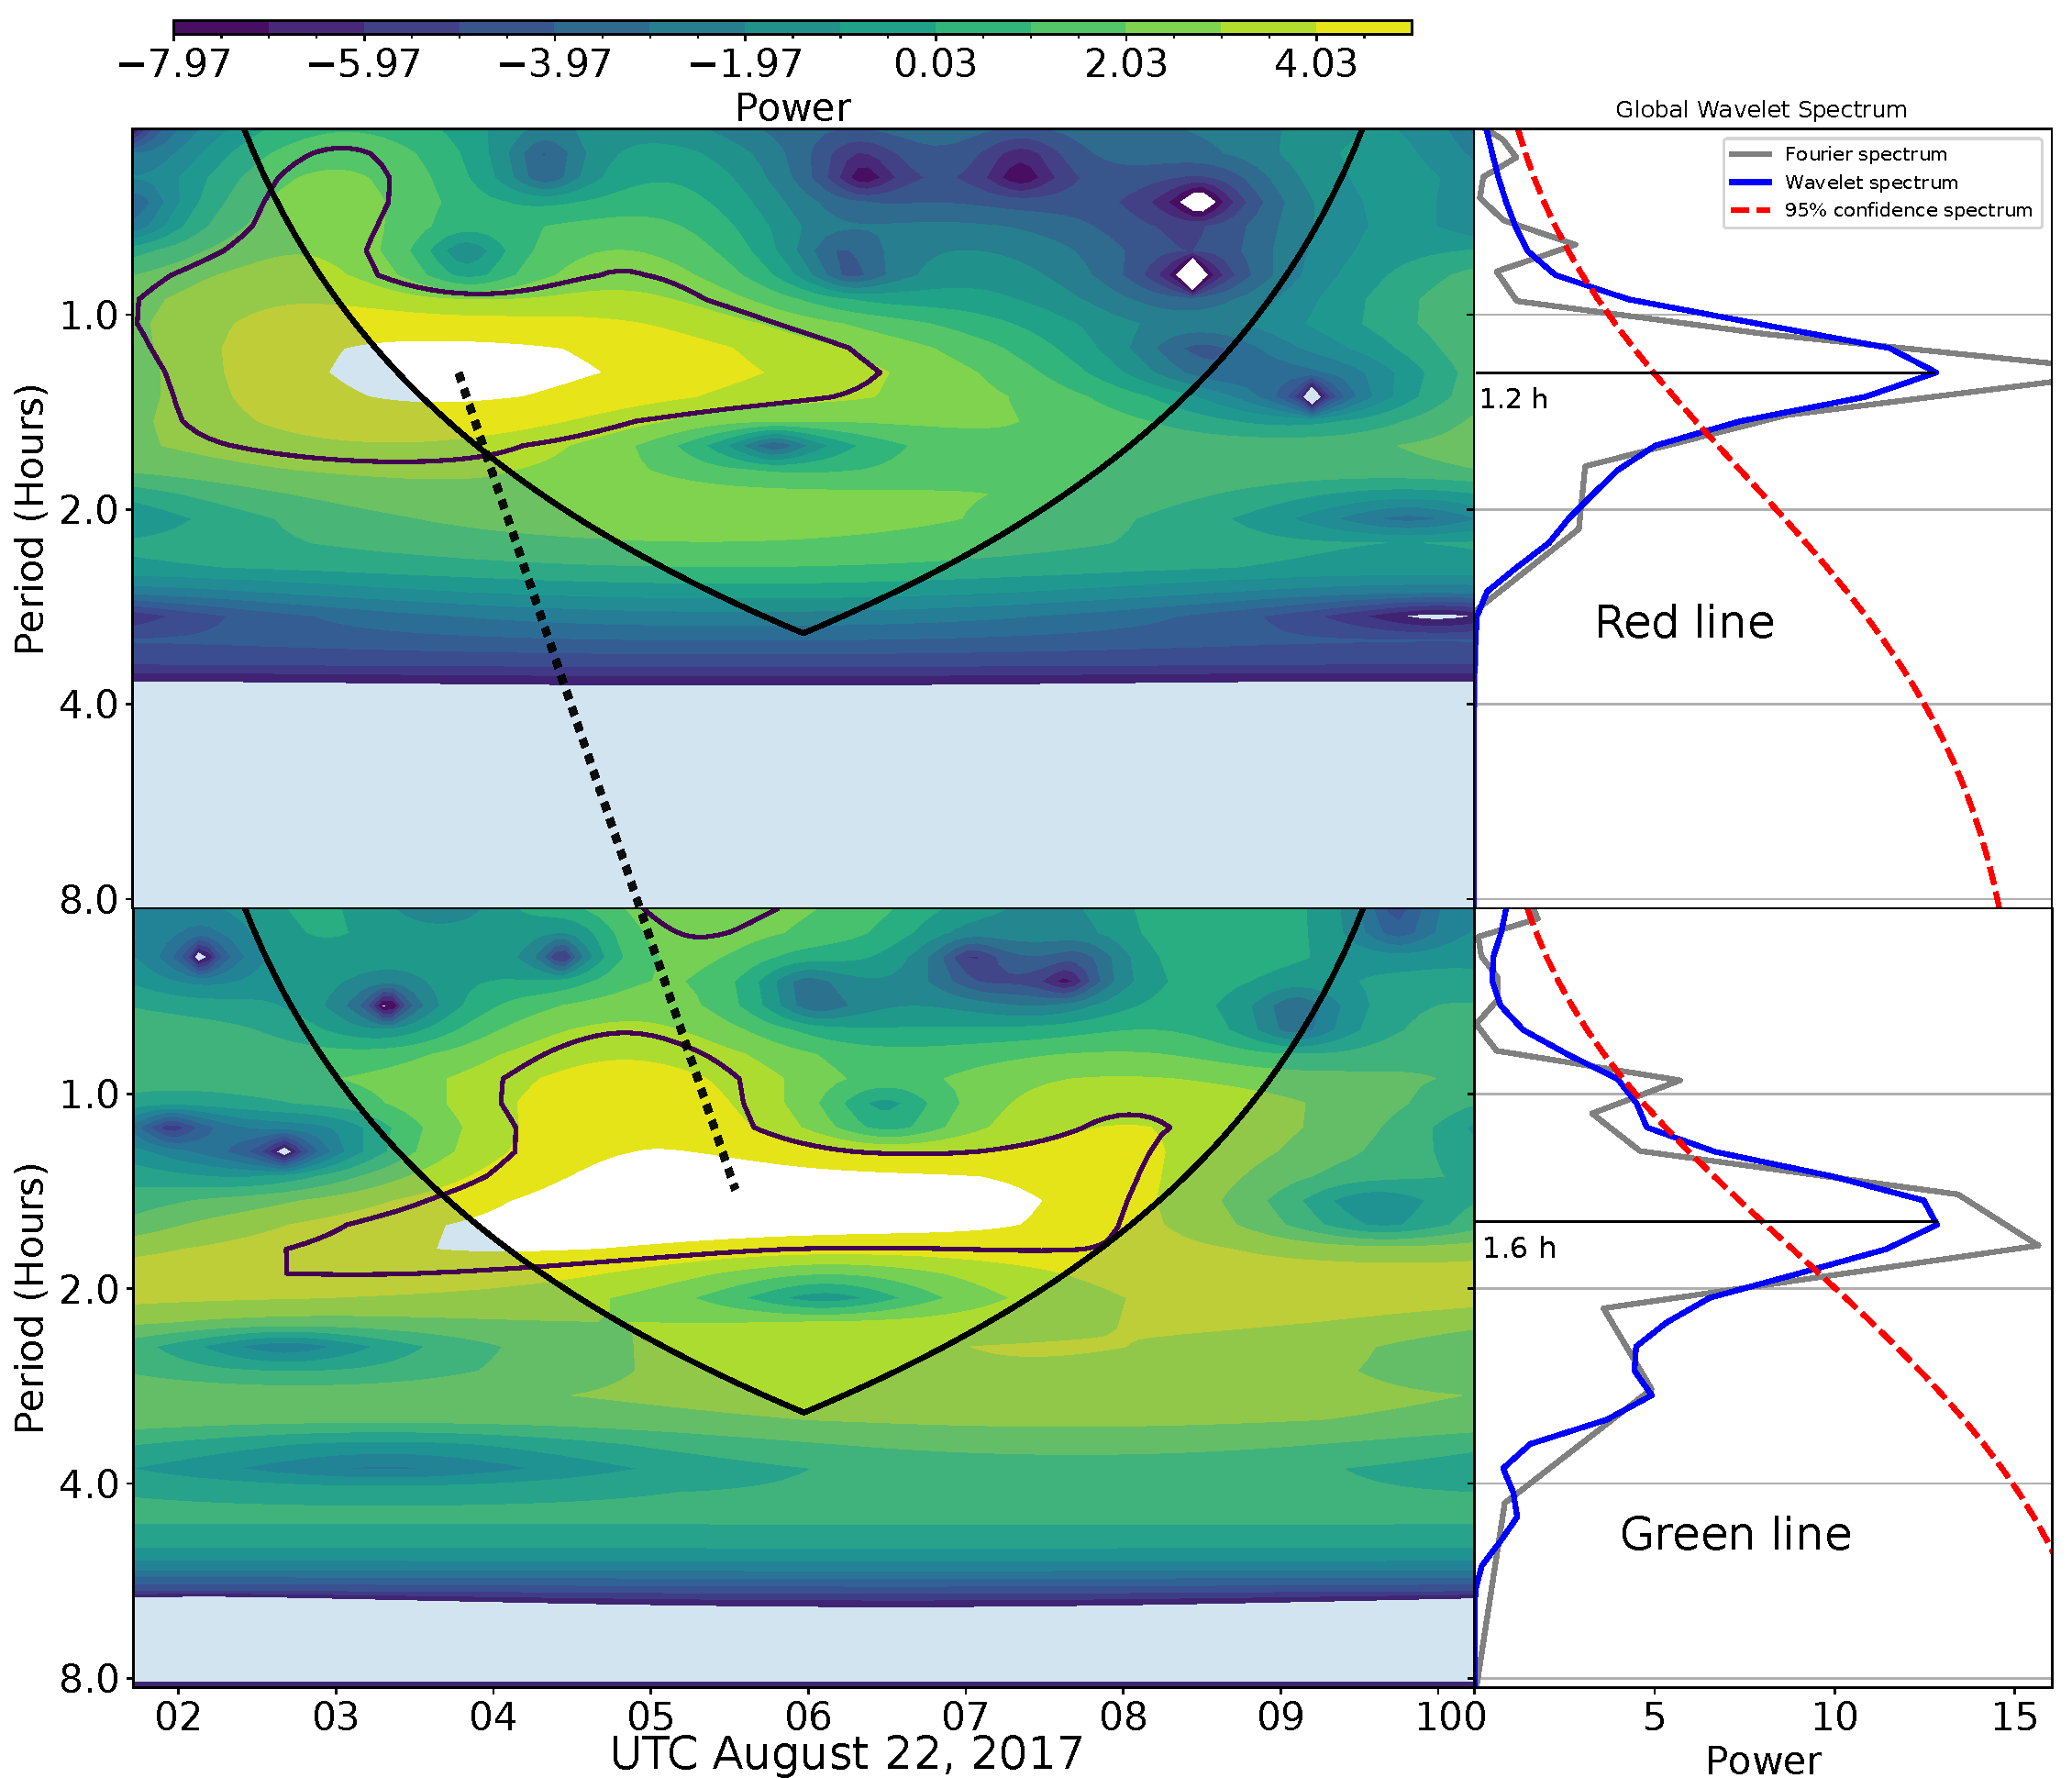
\includegraphics[width=35pc]{wavelet_red_green.pdf}
\caption{Left: Wavelet analyses performed on the de-trended red and the green line brightnesses. The dominant wave time period of 1.3 hour and a similar periodicity of 1.6 hour was found for the red and the green lines, respectively. A dashed-black line is shown to highlight the shift in peak time-periods from the red to the green line. The parabolic black line represents represents the cone of influence, below which the results are unreliable. The 95\% confidence-level powers on the wavelet spectra are represented by the dark-purple contour.  Right: The wavelet power spectrum averaged along all observation times and the corresponding Fast Fourier Transform (FFT) power spectrum and wavelet spectrum are shown in gray and black, respectively. The 95$\%$ confidence interval for the global spectra are shown in red. }
\label{fig:red_green_wv}
\end{figure}
\begin{figure}[H]
	\centering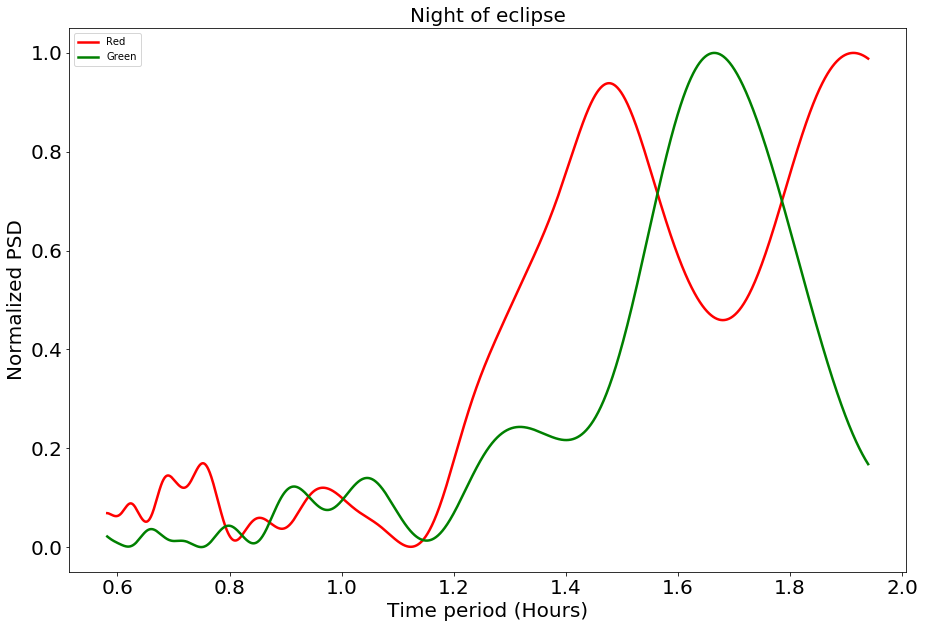
\includegraphics[width=30pc]{lomb.png}
	\caption{Lomb-Scargle periodogram for red and green line on August 22, 2017. Notice the peak time periods on both are similar to that obtained using wavelet method.}
	\label{fig:lomb}
\end{figure}
 
\begin{figure}[H]
\centering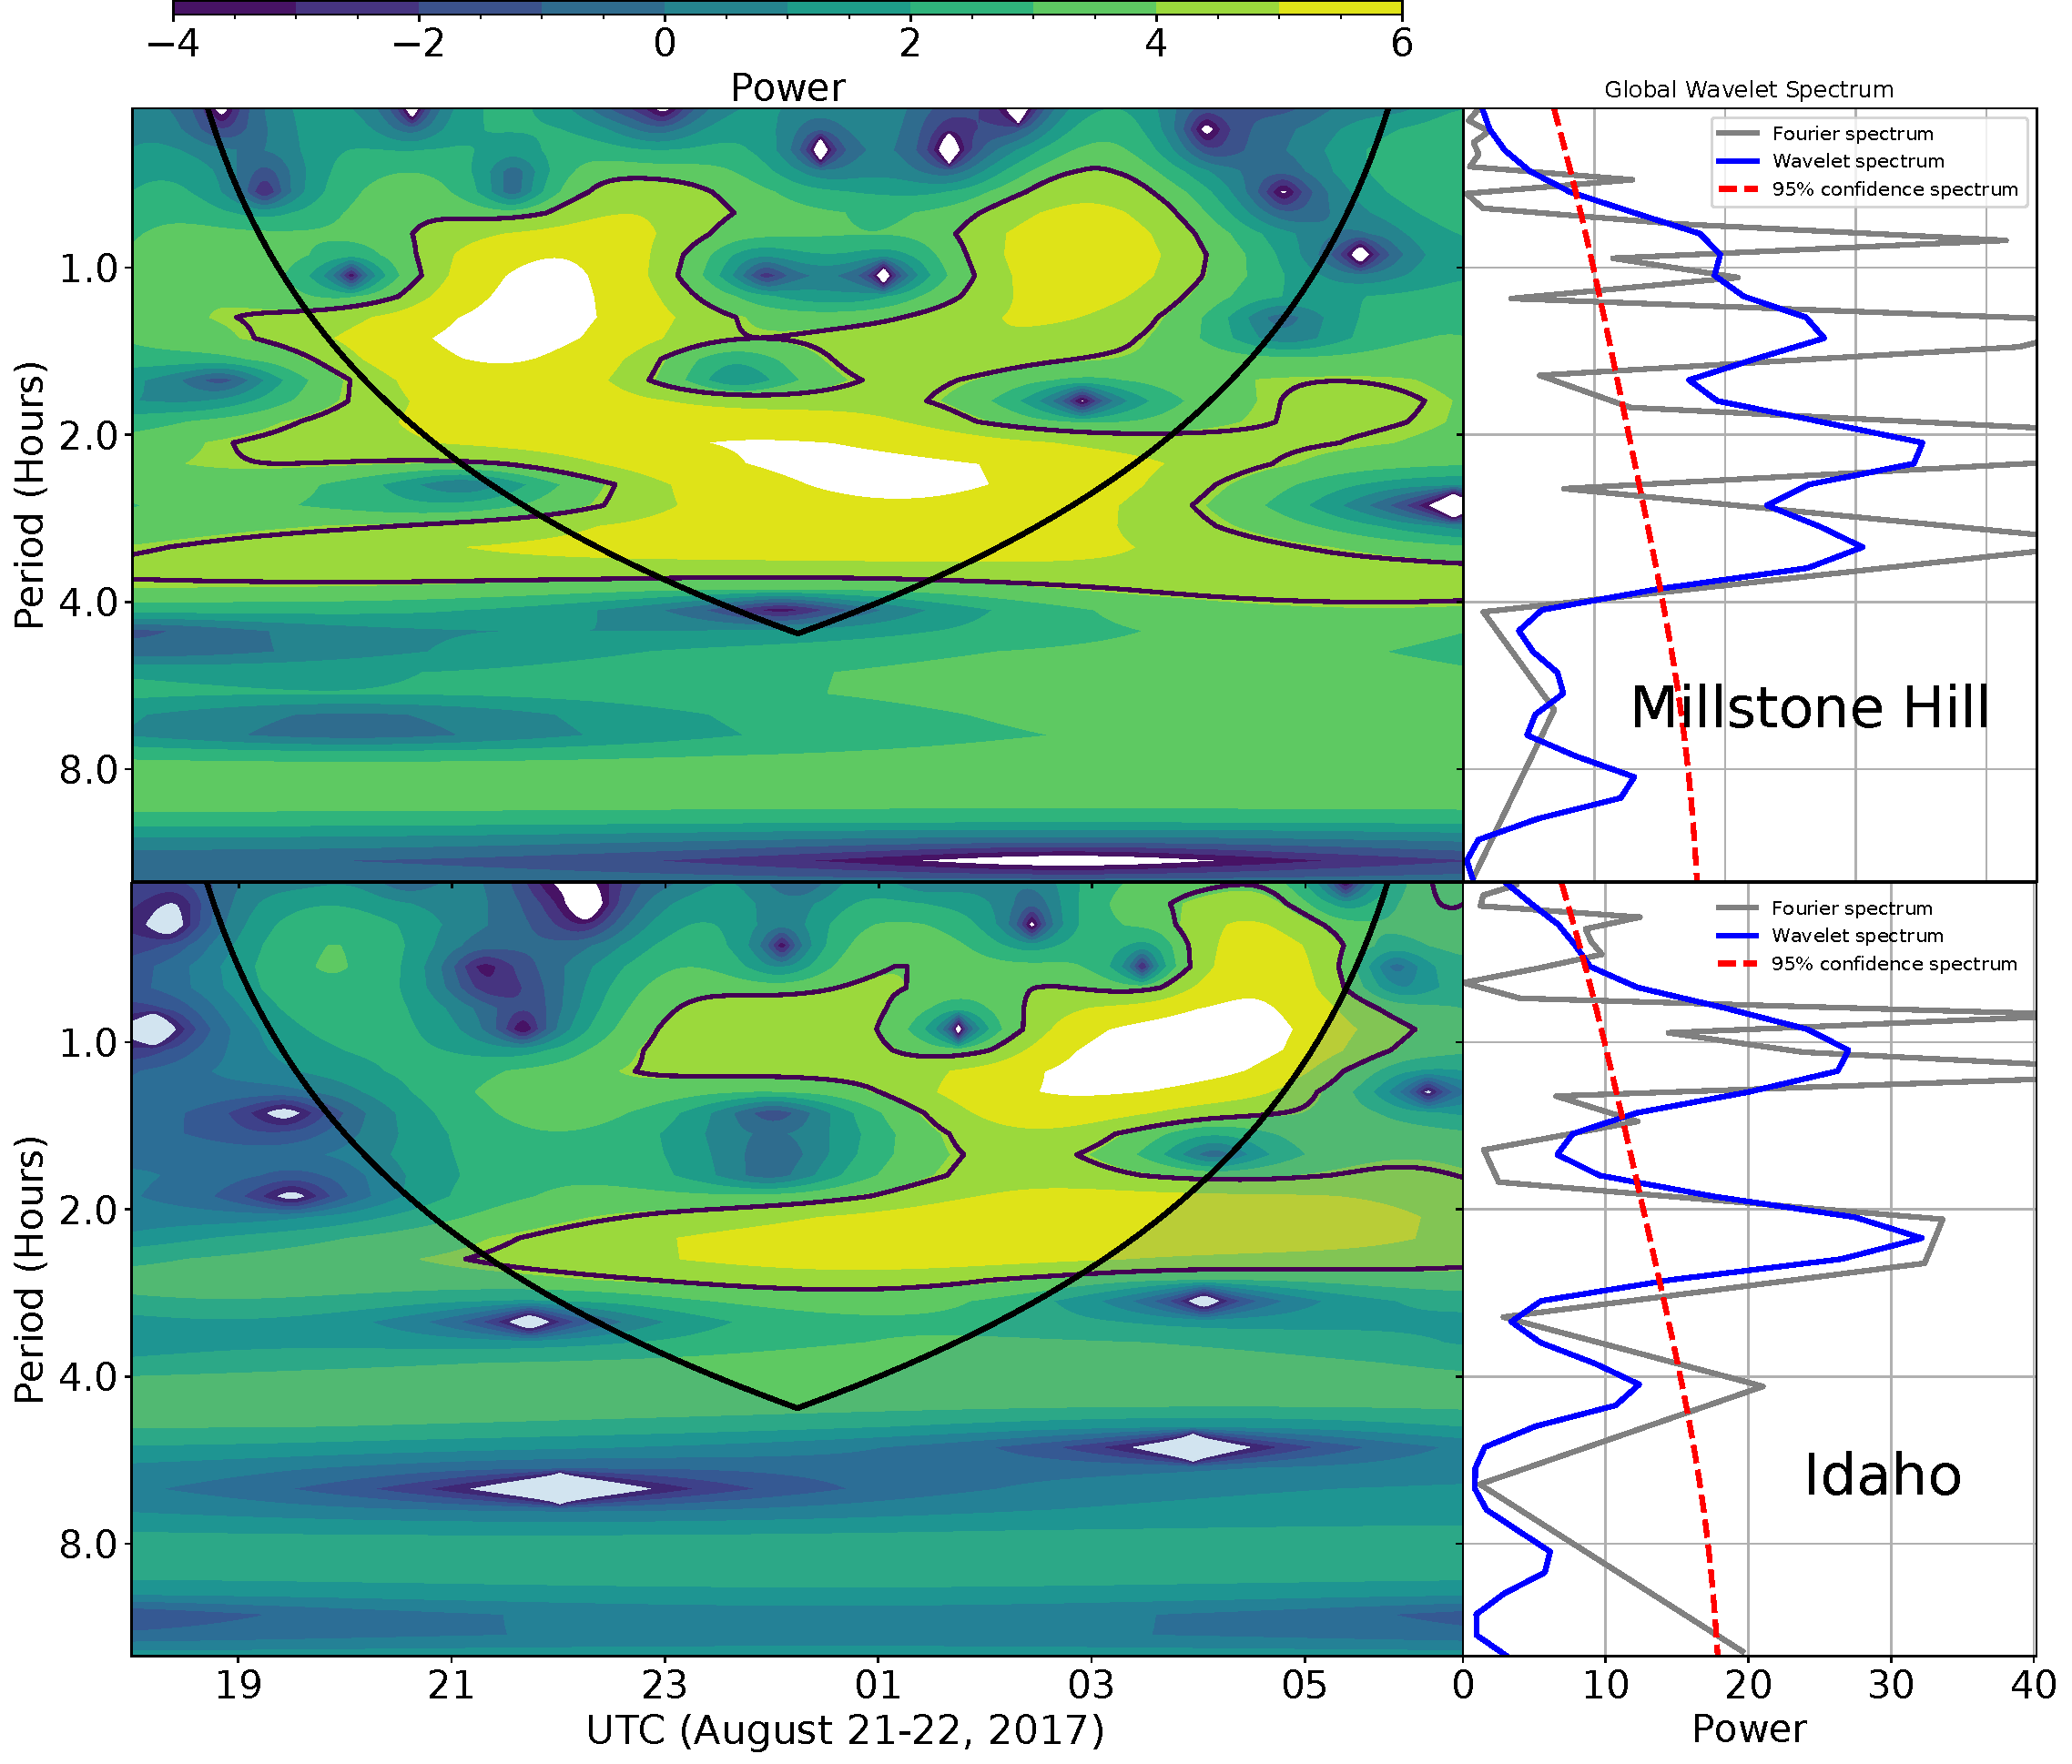
\includegraphics[width=35pc]{muf_digi_wavelet.pdf}
\caption{Left: Wavelet analysis performed on the dynamic part of the MUF profiles from the MH (top) and  INL (bottom). A dominant time period of 1 hour is seen at both locations at different times after midnight UTC most likely associated with the enhancement in AE. Notice wavelet power spectrum with a dominant time period of 1 hour starting around 21~UTC at Millstone Hill which is before the commencement of a minor geomagnetic storm and could be associated with the after effect of the eclipse. }
\label{fig:muf_wv}
\end{figure}
 
\begin{figure}[H]
\centering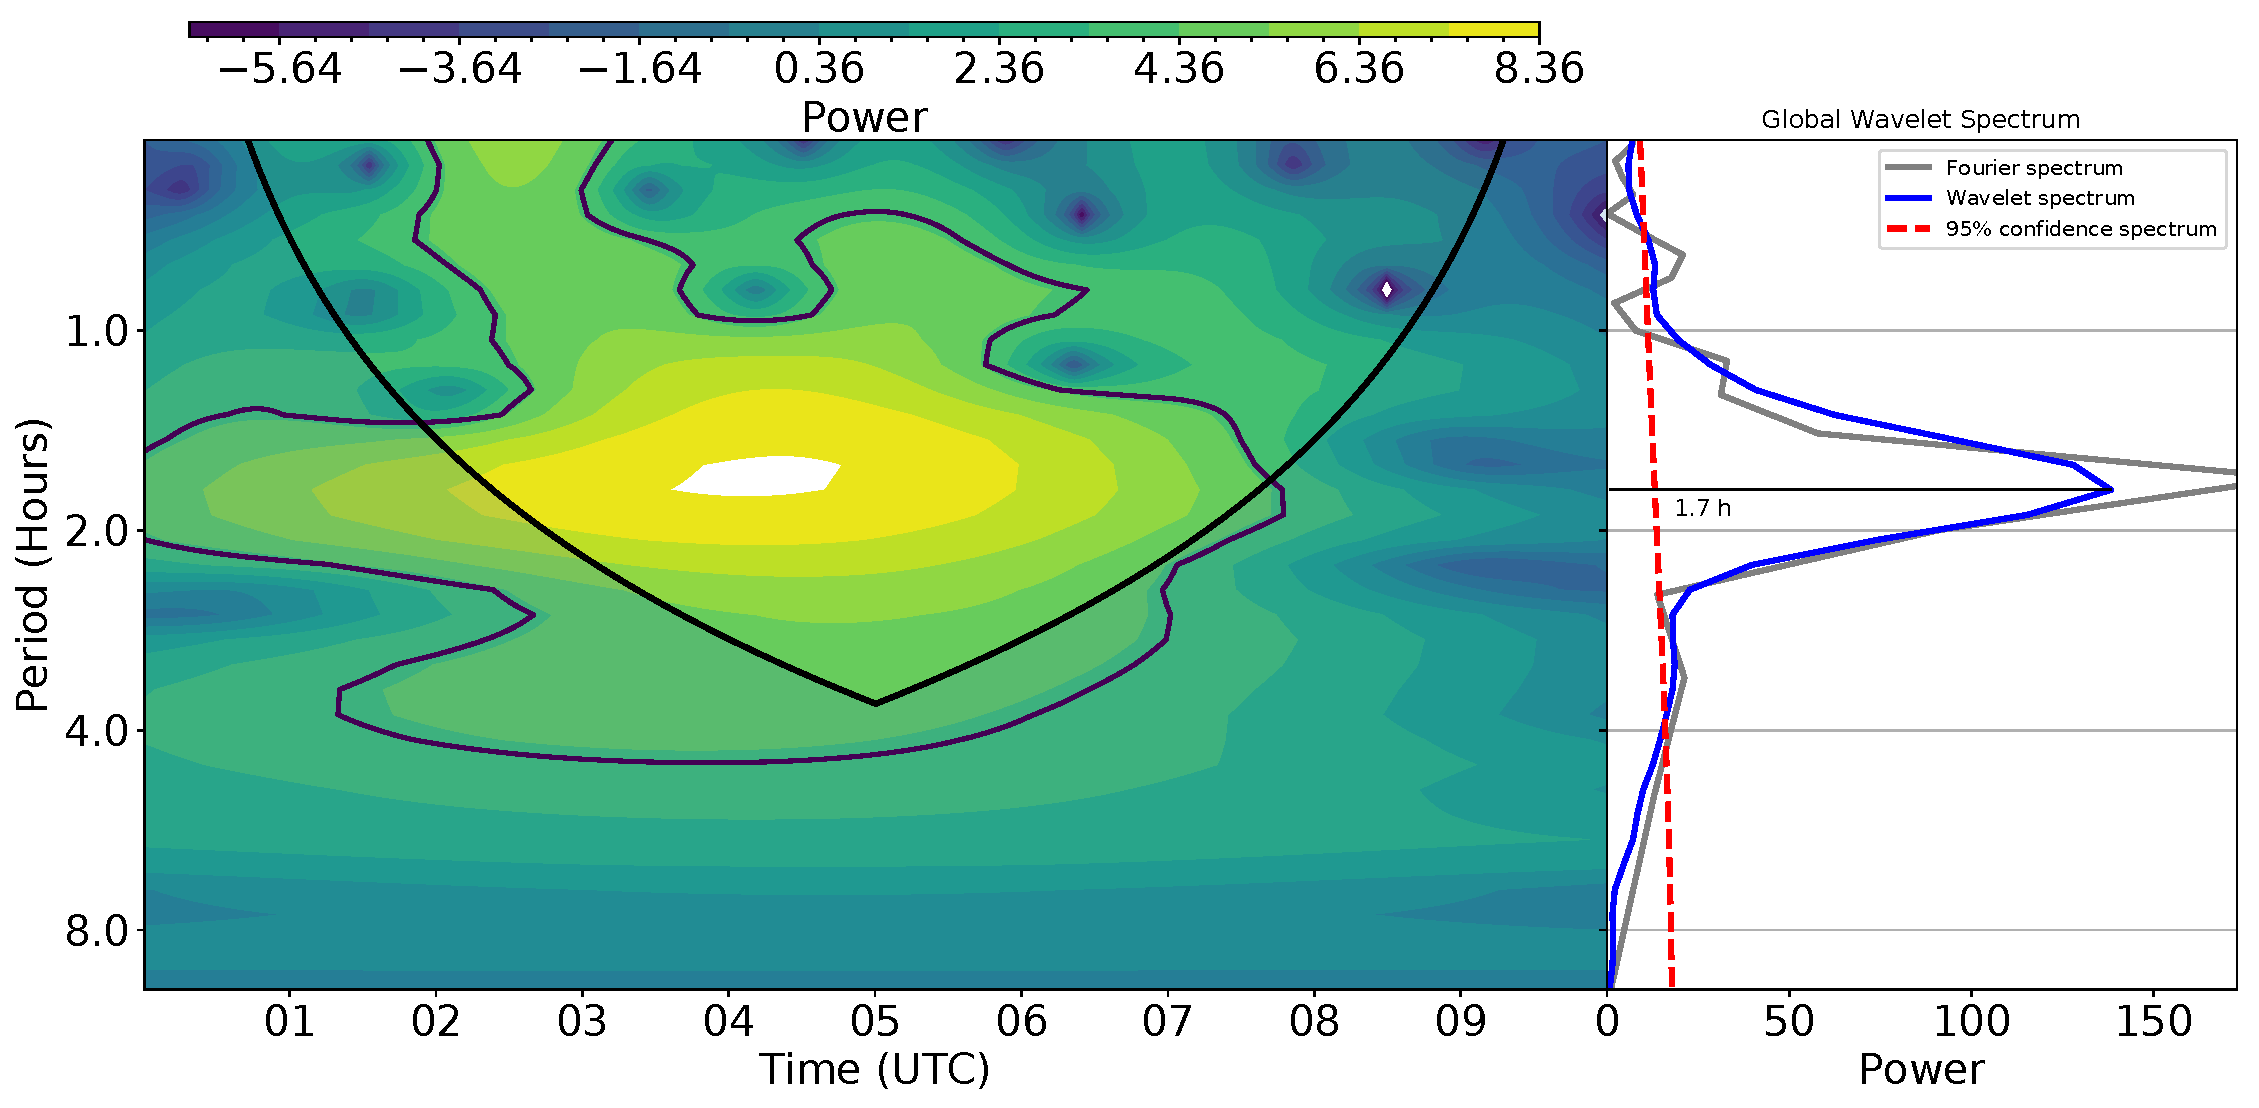
\includegraphics[width=35pc]{dtec.pdf}
\caption{Wavelet analysis performed on the DTEC profile at Carbondale, IL from GPS TEC measurements.  The dominant time period of 1.7 hour is seen starting around 4~UTC.}
\label{fig:wav_tec}
\end{figure} 
 
The vertical phase speed above the spectrograph was found to be 28~m/s estimated using the time delay obtained by cross-correlation analysis on the dynamic part of the red and green line profiles and the difference in their peak altitude (250 km and 123 km, respectively). The vertical wavelength, $\lambda_z$ =152~km, was calculated using the average of the red and the green line dominant wave time periods (1.4 hours) and the vertical phase speed (30~m/s).  

Maps of DTEC is utilized to estimate horizontal wave parameters. Due to a longitudinal structuring of the LSTIDs,  a latitudinal keogram elongated along 120$^\circ$W is utilized and is shown in Figure~\ref{fig:tec_wave}a. The slope of propagation is found to be 10$^\circ$ per 30~minutes, which translate to meridional speed of 616~m/s, equatorward. Similar estimate can also be found at Carbondale, IL, utilizing keogram in Figure~\ref{fig:tecmap}. Spectral analysis~\citep{Mrak2018gw} was applied to the Keogram~\ref{fig:tec_wave}a, to obtain the dominant meridional wavenumbers. The dominant meridional wavenumber is $\sim$0.005~km$^{-1}$ which translates to meridional wavelength $\lambda_m$=1256~km.

\begin{figure}[H]
\centering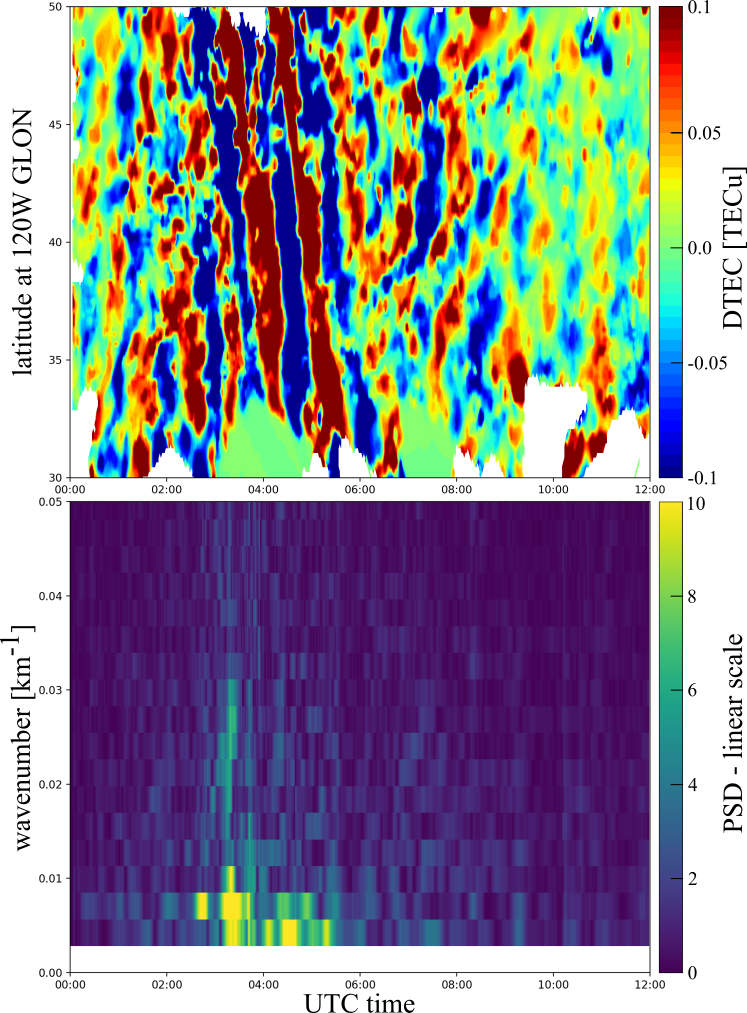
\includegraphics[width=35pc]{wl.png}
\caption{LSTID analysis of meridional propagation velocity at 120$^\circ$W (a), and meridional wavelength utilizing 2D FFT analysis (b).}
\label{fig:tec_wave}
\end{figure} 

\section{Did the Total Solar Eclipse cause the observed LSTIDs}
A total solar eclipse had occurred eight hours earlier before the observed LSTIDs (at Carbondale, IL). While the LSTIDs were most likely generated by geomagnetic effects, the effect of a total solar eclipse on the IT system has also been well-documented by recent and prior studies  \citep[e.g.,][]{coster_gnss_2017,Mrak2018,liu_1998}. Furthermore, the MUF profile at  MH showed perturbations even prior to the start of the geomagnetically active time (Figure \ref{fig:digi}). This could potentially be due to the lingering effect of the eclipse.  
%%% From Ingrid

To test eclipse's effect for our observations, the Global Ionosphere Thermosphere Model (GITM) \citep{ridley_global_2006} was used to simulate the effects of the August 21, 2017 eclipse on the IT system. The Flare Irradiance Spectral Model (FISM; \cite{Chamberlin2007}) was used to specify the solar EUV spectrum, but this was modified to reduce the EUV heating and ionization in the region of the lunar occultation of the Earth to simulate the eclipse effect.
This was done as described by \citet{wu_gitm-data_2018}, although they used a different EUV model. The path of the eclipse was defined in Geocentric Solar Ecliptic (GSE) coordinates as a straight line in the (Y$_{GSE}$, Z$_{GSE}$)-plane, assuming X$_{GSE}$ constant. The reduction in EUV irradiance was based on the distance between each GITM grid point and the center of totality; at the center of totality, the EUV irradiance was reduced to 10\% of the normal value, which linearly increased until the edge of the occultation region was approached, after which the EUV increased exponentially back to 100\% at 3,800 km distance from the center of totality.
% * <temujinparuhang@gmail.com> 2018-10-02T19:30:55.601Z:
% 
% > This was done as described by \citet{wu_gitm-data_2018}, although they used a different EUV model.
% Any reference to what the EUV model used?
% 
% ^ <icnossen@googlemail.com> 2018-10-09T12:04:34.743Z:
% 
% I've added this to the text. The full reference is:
% ^ <temujinparuhang@gmail.com> 2018-10-29T15:49:10.678Z.

%
% ^.
Two simulations were run; one with the eclipse event included, and, one without for comparison (the control simulation). Both simulations were otherwise set up identically. The model was run with a resolution of 2.0$^\circ$ in latitude, 4.0$^\circ$ in longitude, and $\sim$0.3 times the scale height in altitude, spanning from 100 km to approximately 600 km altitude. Observed solar wind and interplanetary magnetic field data were used to drive the high-latitude electric potential and auroral precipitation patterns. The simulations used here are the same as those analyzed by Cnossen et al. [in preparation], where the simulation setup is described in further detail. 
   \begin{figure}[H]
 \centering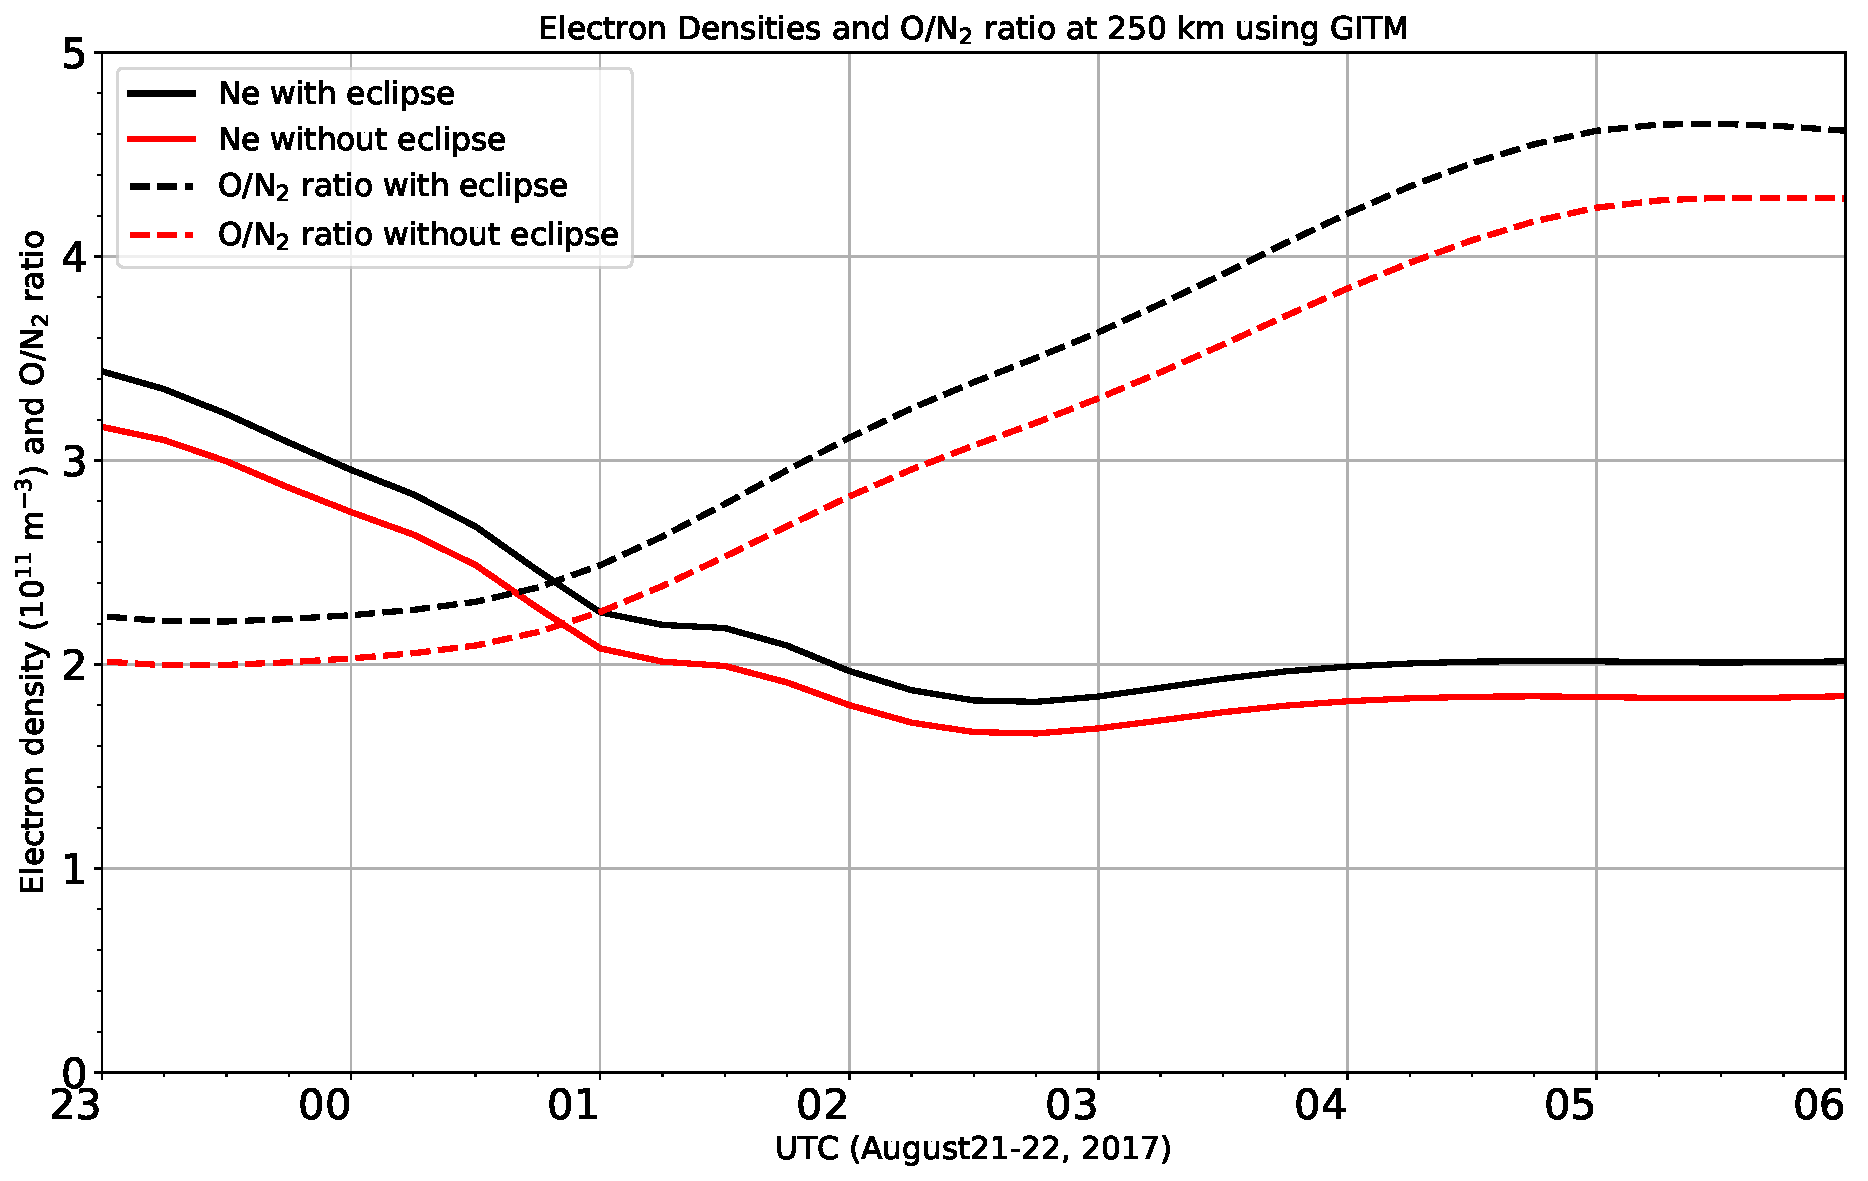
\includegraphics[width=35pc]{ec_vs_nec_tid.pdf}
 \centering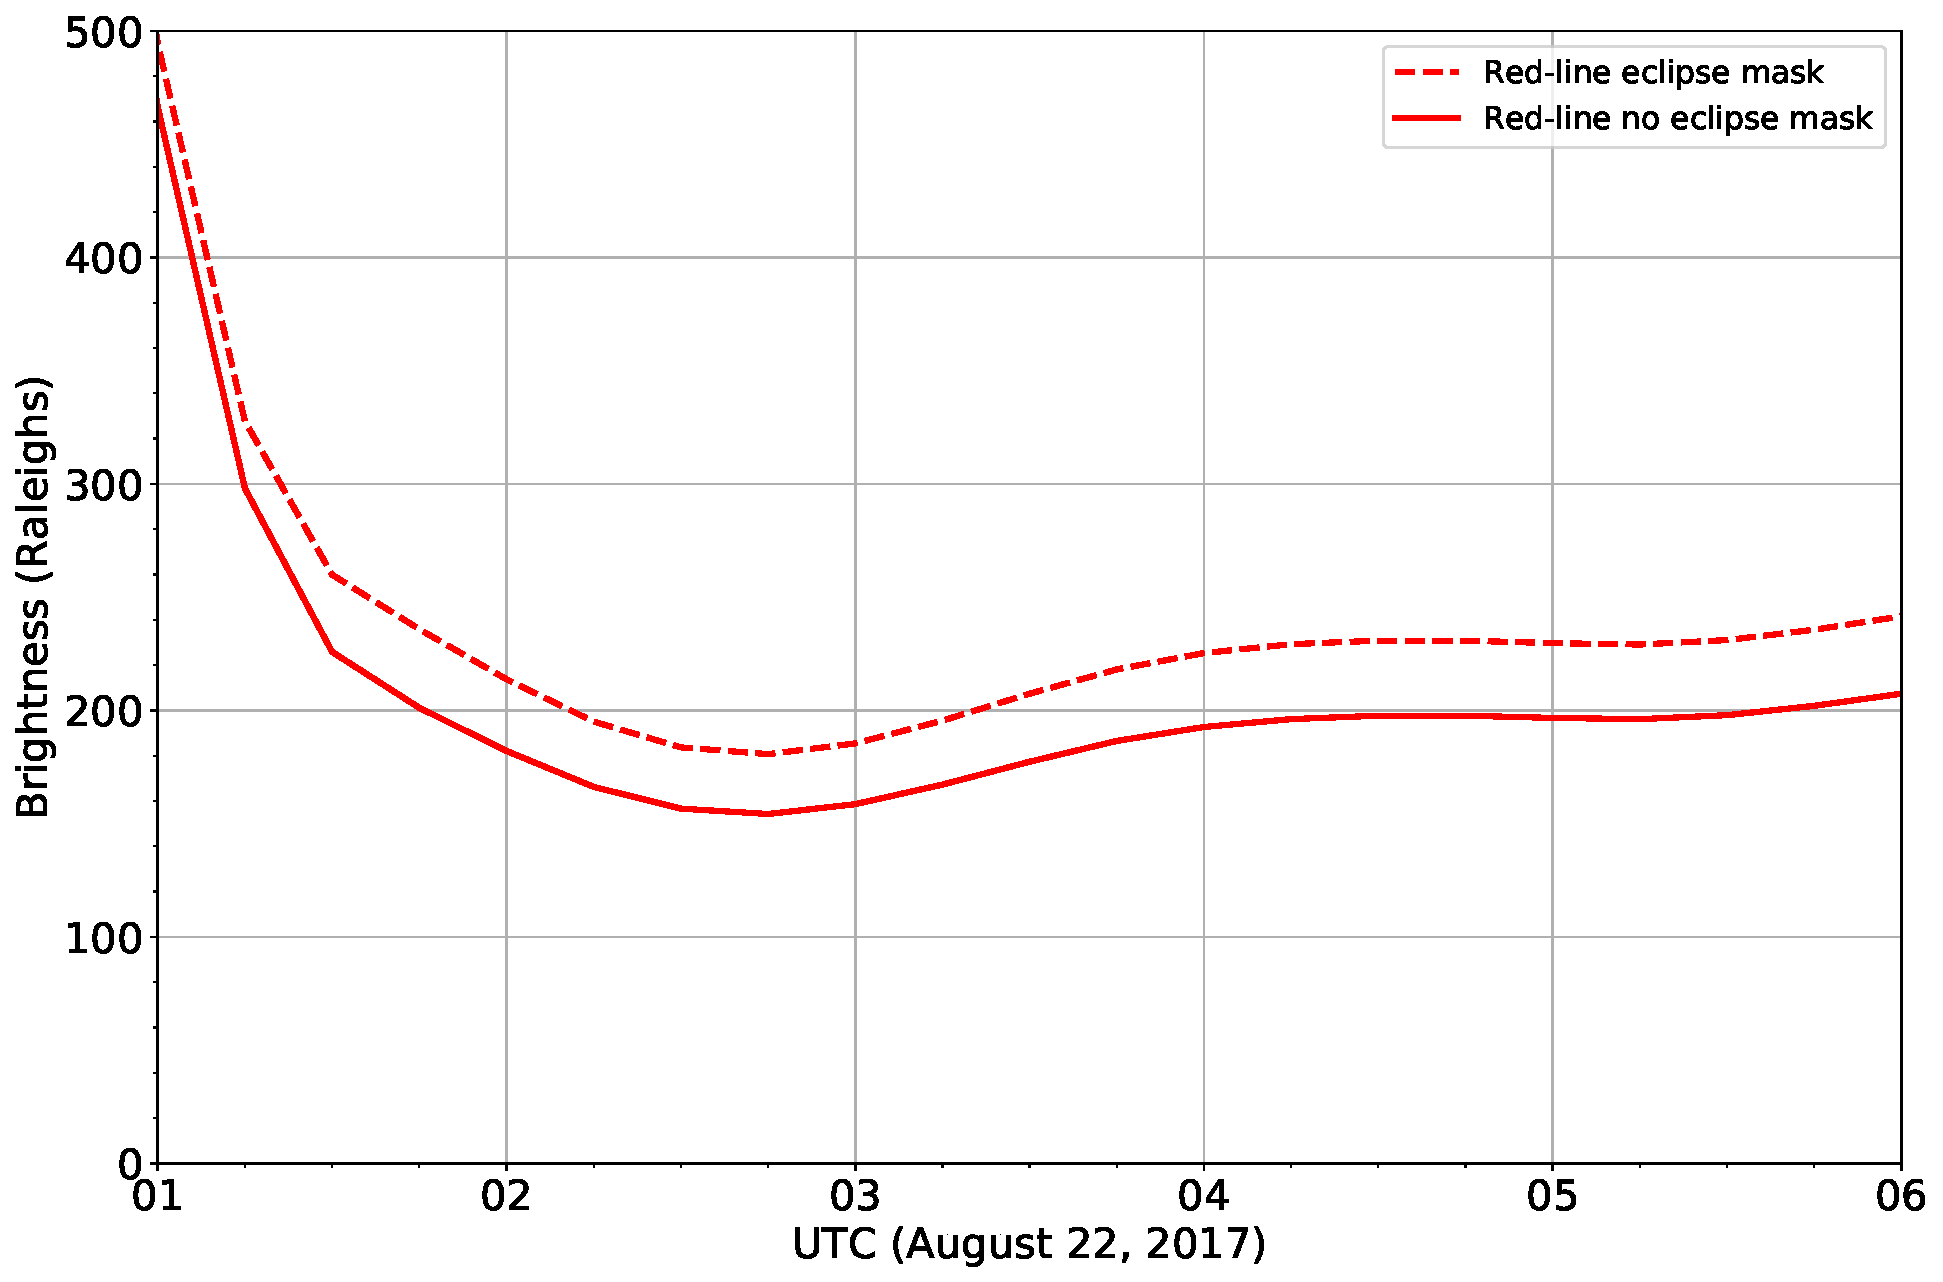
\includegraphics[width=30pc]{GITM_with_GLOW_dglow.pdf}
 \caption{ Electron densities  and the thermospheric O/N$_2$ ratio at 250 km (peak of red line emission) using an EUV mask to mimic the effect of a total solar eclipse, and no-eclipse conditions (but including geomagnetic effects) using the GITM model at Carbondale, IL. Notice that while the profiles are very similar, both electron density and the O/N$_2$ ratios are $\sim$ 10\% higher when the effects due the eclipse were considered. }
 \label{fig:ec_ne}
 \end{figure}
 
 %%%%%
 
   \begin{figure}[H]
 %\centering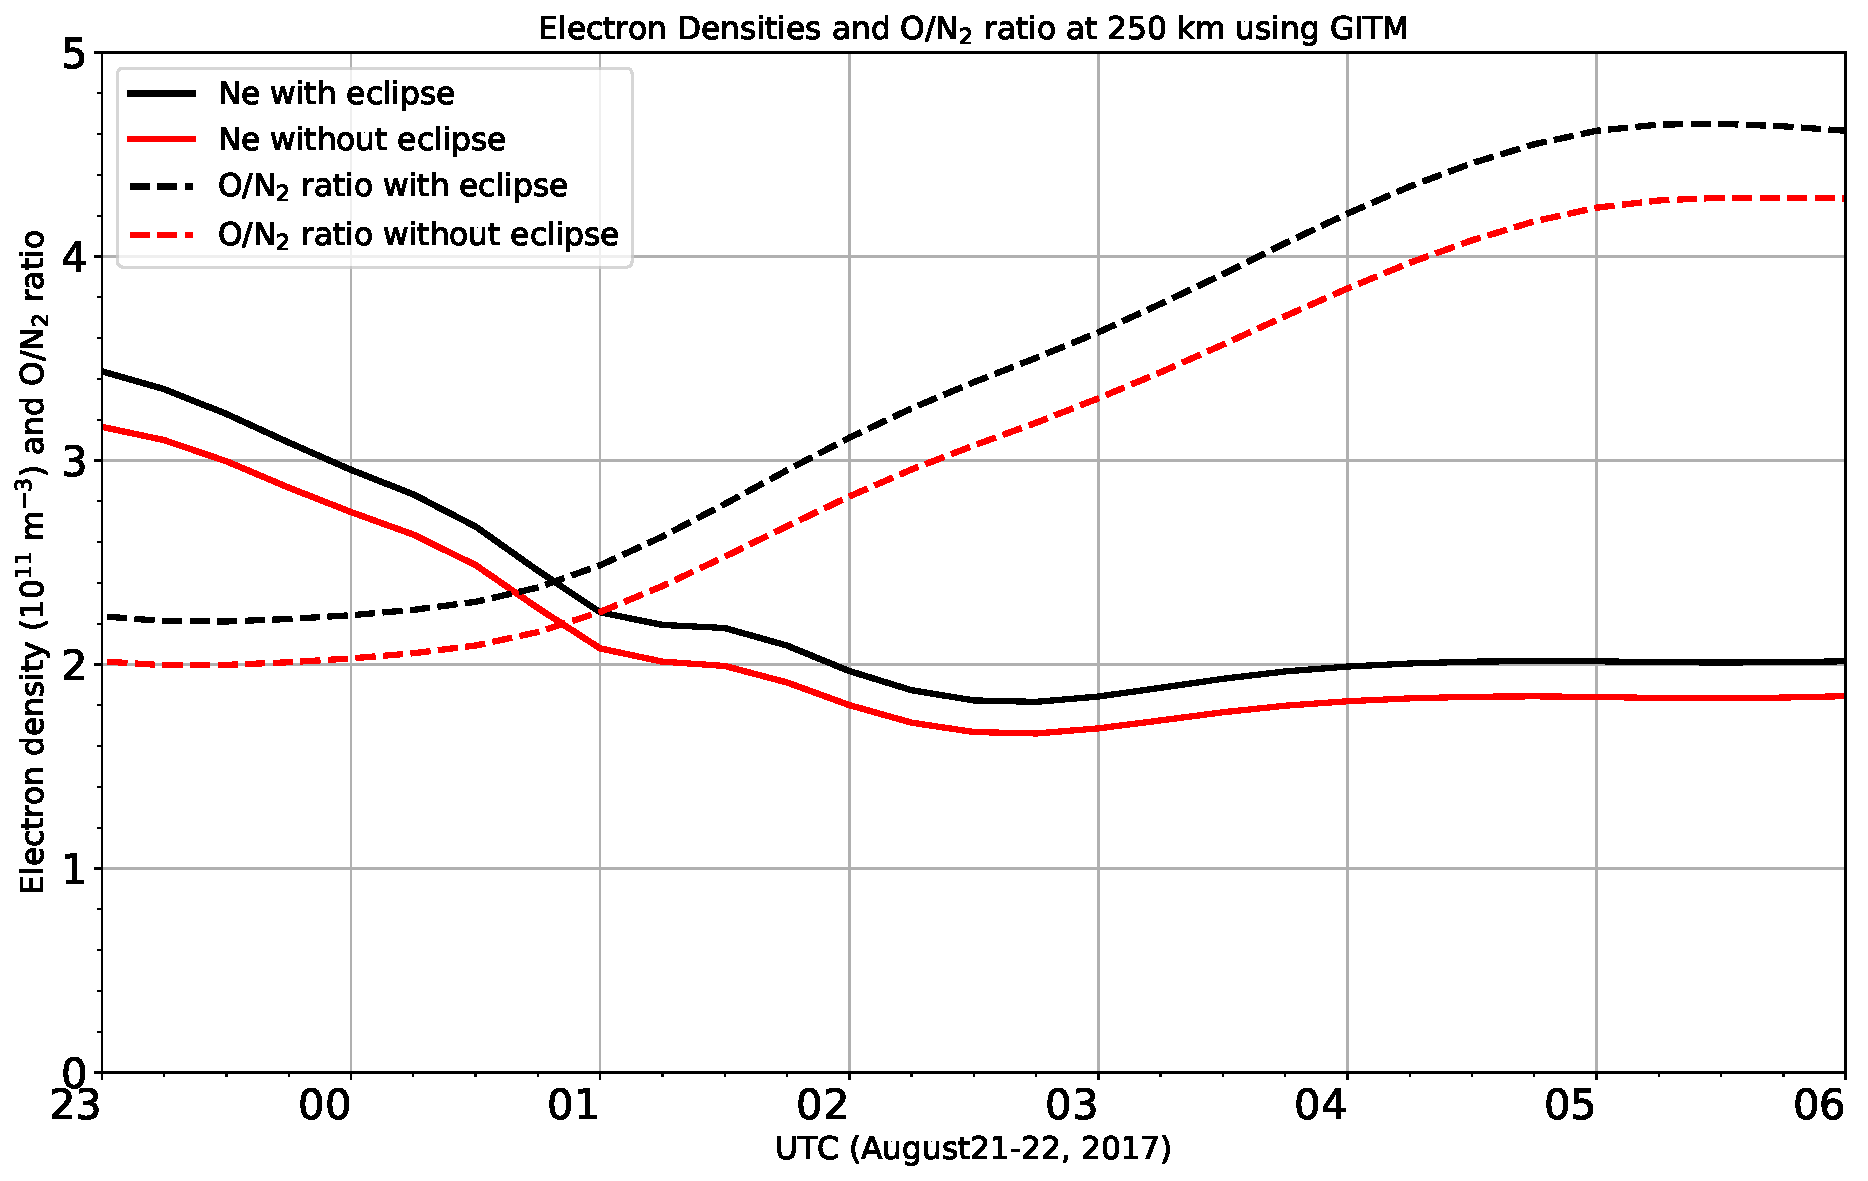
\includegraphics[width=35pc]{ec_vs_nec_tid.pdf}
 \centering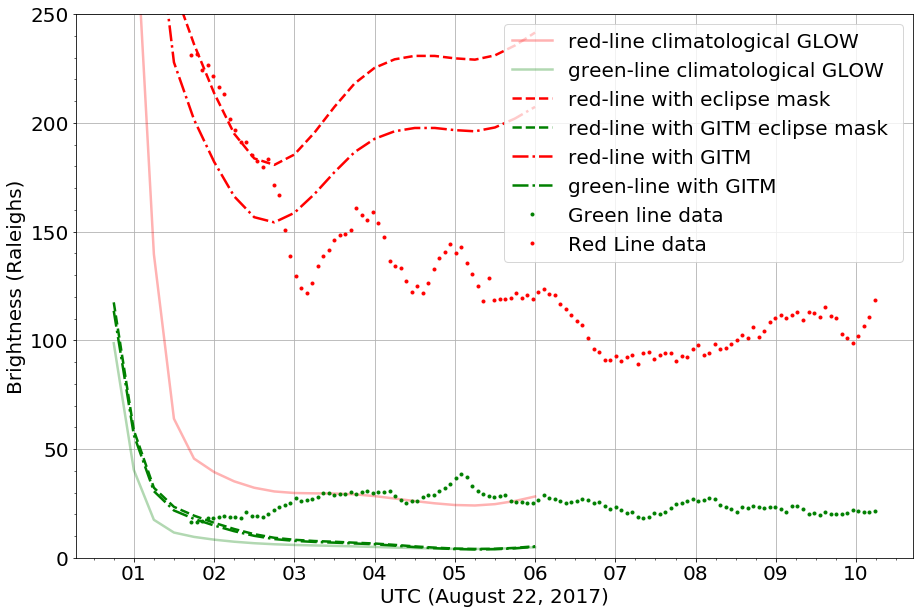
\includegraphics[width=30pc]{GITM_with_GLOW_dglow.png}
 \caption{ Electron densities  and the thermospheric O/N$_2$ ratio at 250 km (peak of red line emission) using an EUV mask to mimic the effect of a total solar eclipse, and no-eclipse conditions (but including geomagnetic effects) using the GITM model at Carbondale, IL. Notice that while the profiles are very similar, both electron density and the O/N$_2$ ratios are $\sim$ 10\% higher when the effects due the eclipse were considered. }
 \label{fig:glow_est}
 \end{figure}
 
% * <icnossen@googlemail.com> 2018-09-24T11:26:01.141Z:
% 
% > To test this further the Global Ionosphere Thermosphere Model (GITM) \citep{ridley_global_2006} was used to simulate the effects of the August 21, 2017 eclipse on the IT system. To do this, GITM was modified to reduce the EUV heating and ionization in the region of the moon occultation of the Earth. This was done as described by \citet{wu_gitm-data_2018}, although they used a different EUV model. The path of the eclipse was defined in Geocentric Solar Ecliptic (GSE) coordinates as a straight line in the (Y$_{GSE}$, Z$_{GSE}$)-plane, assuming X$_{GSE}$ constant. The reduction in EUV irradiance was based on the distance between each GITM grid point and the center of totality: at the center of totality, the EUV irradiance was reduced to 10\% of the normal value, which linearly increased until the edge of the occultation region was approached, after which the EUV increased exponentially back to 100\% at 3,800 km distance from the center of totality.
% > Two simulations were run: one with the eclipse event included and one without for comparison (the control simulation). Both simulations were otherwise set up identically. The model was run with a resolution of 0.5$^\circ$ in latitude, 2.0$^\circ$ in longitude, and $\sim$0.3 times the scale height in altitude, spanning from 100 km to approximately 600 km altitude. Observed solar wind and interplanetary magnetic field data were used to drive the high-latitude electric potential and auroral precipitation patterns. The simulations used here are the same as those analyzed by Cnossen et al. [in preparation], who describe the simulation setup in further detail. 
% This is a methodology description, so you could consider making a separate section for this, before presenting the results. This could be a separate "model simulations" section on the same level as the "data" section, or you could make a "methodology" section, with subsections for the different data sources and the model simulation description. It's up to you, but I think it works better to keep the methodology separate from the actual results.
% 
% ^ <temujinparuhang@gmail.com> 2018-10-03T23:54:23.973Z:
% 
% I have made a separate section for it but not sure if the title represents that, open to title name suggestions
%
% ^ <icnossen@googlemail.com> 2018-10-09T12:51:10.324Z:
% 
% I think the organization could work this way and the title is fine by me.
%
% ^ <temujinparuhang@gmail.com> 2018-10-29T15:49:20.142Z.
% The electron transport model, GLOW \citep{solomon_1988,solomon1989630,bailey2002}, was used to estimate the red and green line brightnesses based on climatological and GITM derived inputs. 
%%%%%%%%%%%%%

Figure \ref{fig:ec_ne} shows the electron density and  the thermospheric O/N$_2$ ratios estimated using GITM at 250 km, which is where the red line emission peaks, for the two cases: with and without the effect of the eclipse. Both the electron density and the O/N$_2$ ratio were around 10\% higher when the the eclipse's effect were included but the time profile was very similar to the non-eclipse case. Figure \ref{fig:ec_ne} (bottom) shows GLOW model brightness estimates using GITM inputs (both with and without eclipse's effect). The red and the green line brightnesses scaled to the climatological GLOW estimates the night before (assumed to have no disturbances) plus the climatological GLOW brightness estimates are also shown for comparison. GLOW's brightness estimates for the red line using GITM's inputs  with eclipse's effect are comparable to the data until the brightness perturbations occur ($\sim$ 0300 UTC). While these simulation results imply that the eclipse enhanced the TID strength, no conclusion on the possibility of the eclipse contributing to the formation of the observed TIDs could be drawn.  

\section{Discussion}
The dynamic part of the red and green lines and the DTEC profiles at Carbondale, IL, coincided better from 3--6~UTC (August 22, 2017, Figure \ref{fig:dtec_carb} ), which is also when the DTEC keogram show prominent LSTIDs (Figure \ref{fig:tecmap}, bottom). All of the wavelet spectra have a similar dominant wave power around the same time frame (3--6 UTC). In addition, the AE index peaks and recovers during the same time period too (Figure \ref{fig:gindx}). This indicates that the increase in auroral currents and associated Joule heating near the poles were responsible for the observed LSTIDs. There are TIDs prior to and after 3--6 UTC in the DTEC map (Figure \ref{fig:tecmap}, bottom); however, their scale are sizes smaller and and the strength is weaker. 

The estimated dominant wave time-periods are slightly different for different observations, i.e., 1.3$\pm$0.5, 1.6$\pm$0.8 and 1.7$\pm$0.7 h for the red line, green line and DTEC, respectively at Carbondale, IL. The dominant wave period of around 1h was also found for MUF profiles at both INL and MH. MUF is sensitive to the bottom-side ionospheric plasma densities, the red and green line brightnesses are sensitive to both the plasma and the neutral densities at the altitude they peak at, and the TEC measurements are sensitive to the line of sight ionospheric plasma density. These differences could explain the discrepancy in dominant time periods. 

Previous studies have observed disturbances in the IT system well after the eclipse and far away from its path \citep[e.g,][]{harding_nightside_eclipse,eclipse_belg}. \citet{goncharenko_mh_hill_eclipse} reported enhanced electron density (> 50-150\%) starting from 21~UTC, August 21, 2017 to at least midnight UTC (August 22) based on radar measurements at MH hours after the eclipse.  The authors attributed this enhancement in electron density to the downward flux of plasma from the plasmasphere that was filled by upwelling of plasma immediately following the eclipse. This electron density enhancement was not predicted by GITM, as it does not include contributions from the plasmasphere. 21--22~UTC is also when one of the peaks in MUF wavelet spectrum with a dominant wave time-period of around 1h at MH is observed (Figure \ref{fig:muf_wv} ). This indicates that the observed perturbation in MUF was caused by eclipse related effect with similar time period of around 1h that was observed later with the geomagnetic effect. \citet{wu_gitm-data_2018} reported that the IT system's response to the eclipse in GITM decays much quicker than is seen in TEC and NmF2 observations. On the other hand, a 10\% increase in both O/N$_2$ ratio and N$_e$ at Carbondale, IL predicted by GITM is consistent with the quantitative enhancement in the observed red line brightness observed when compared to the night before (see Figure\ref{fig:supp} ). However, GITM failed to produce the wave-like perturbations seen red and green line airglow brightnesses, possibly due coarser resolution in latitude and longitude. Thus, it is possible that eclipse's long-term effect not only influenced the TID strength, but also could have interacted with the geomagnetic effects in the formation of the observed LSTIDs. Based on this study it can only be concluded that the eclipse's effect only enhanced the TID's strength. 
% * <temujinparuhang@gmail.com> 2018-10-29T23:33:09.191Z:
% 
% > However, GITM failed to produce the wave-like perturbations seen red and green line airglow brightnesses, possibly due coarser resolution in latitude and longitude
% Might have to re-word this open to suggestion
% 
% ^.
% * <icnossen@googlemail.com> 2018-10-09T13:54:40.491Z:
% 
% > ; however, no conclusion on that could be drawn based on this study
% In that case it should not be listed as a key point.
% 
% ^ <temujinparuhang@gmail.com> 2018-10-29T23:23:56.232Z:
% 
% Re worded this part to make it sound in non-formal terms : "the eclipse influnced the TID strength, but we dont know if the eclipse induced pre-conditioning helped in the formation of the TID"
%
% ^.

  \begin{figure}[H]
 \centering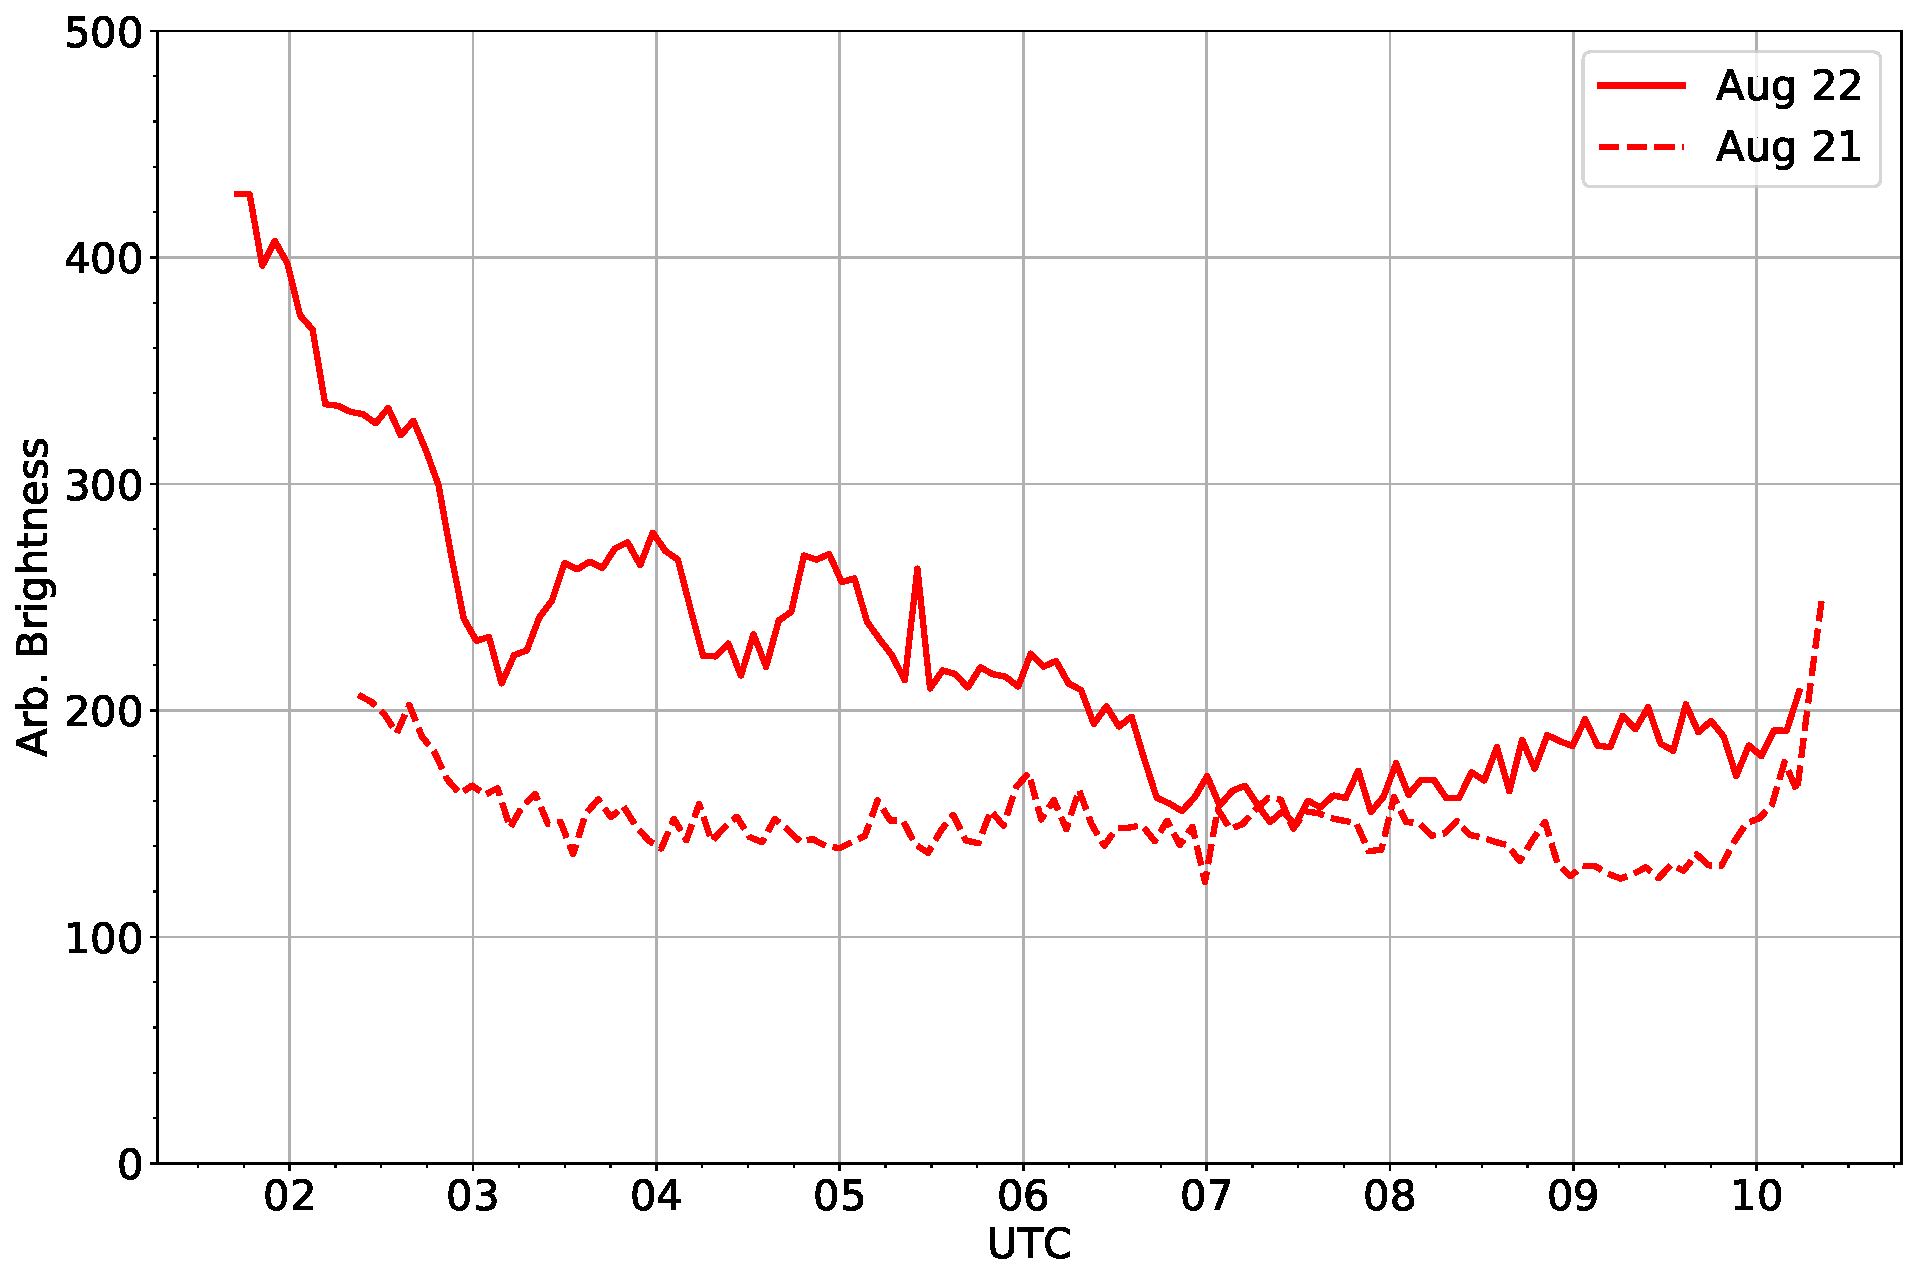
\includegraphics[width=35pc]{supplimentary1.pdf}
 %\centering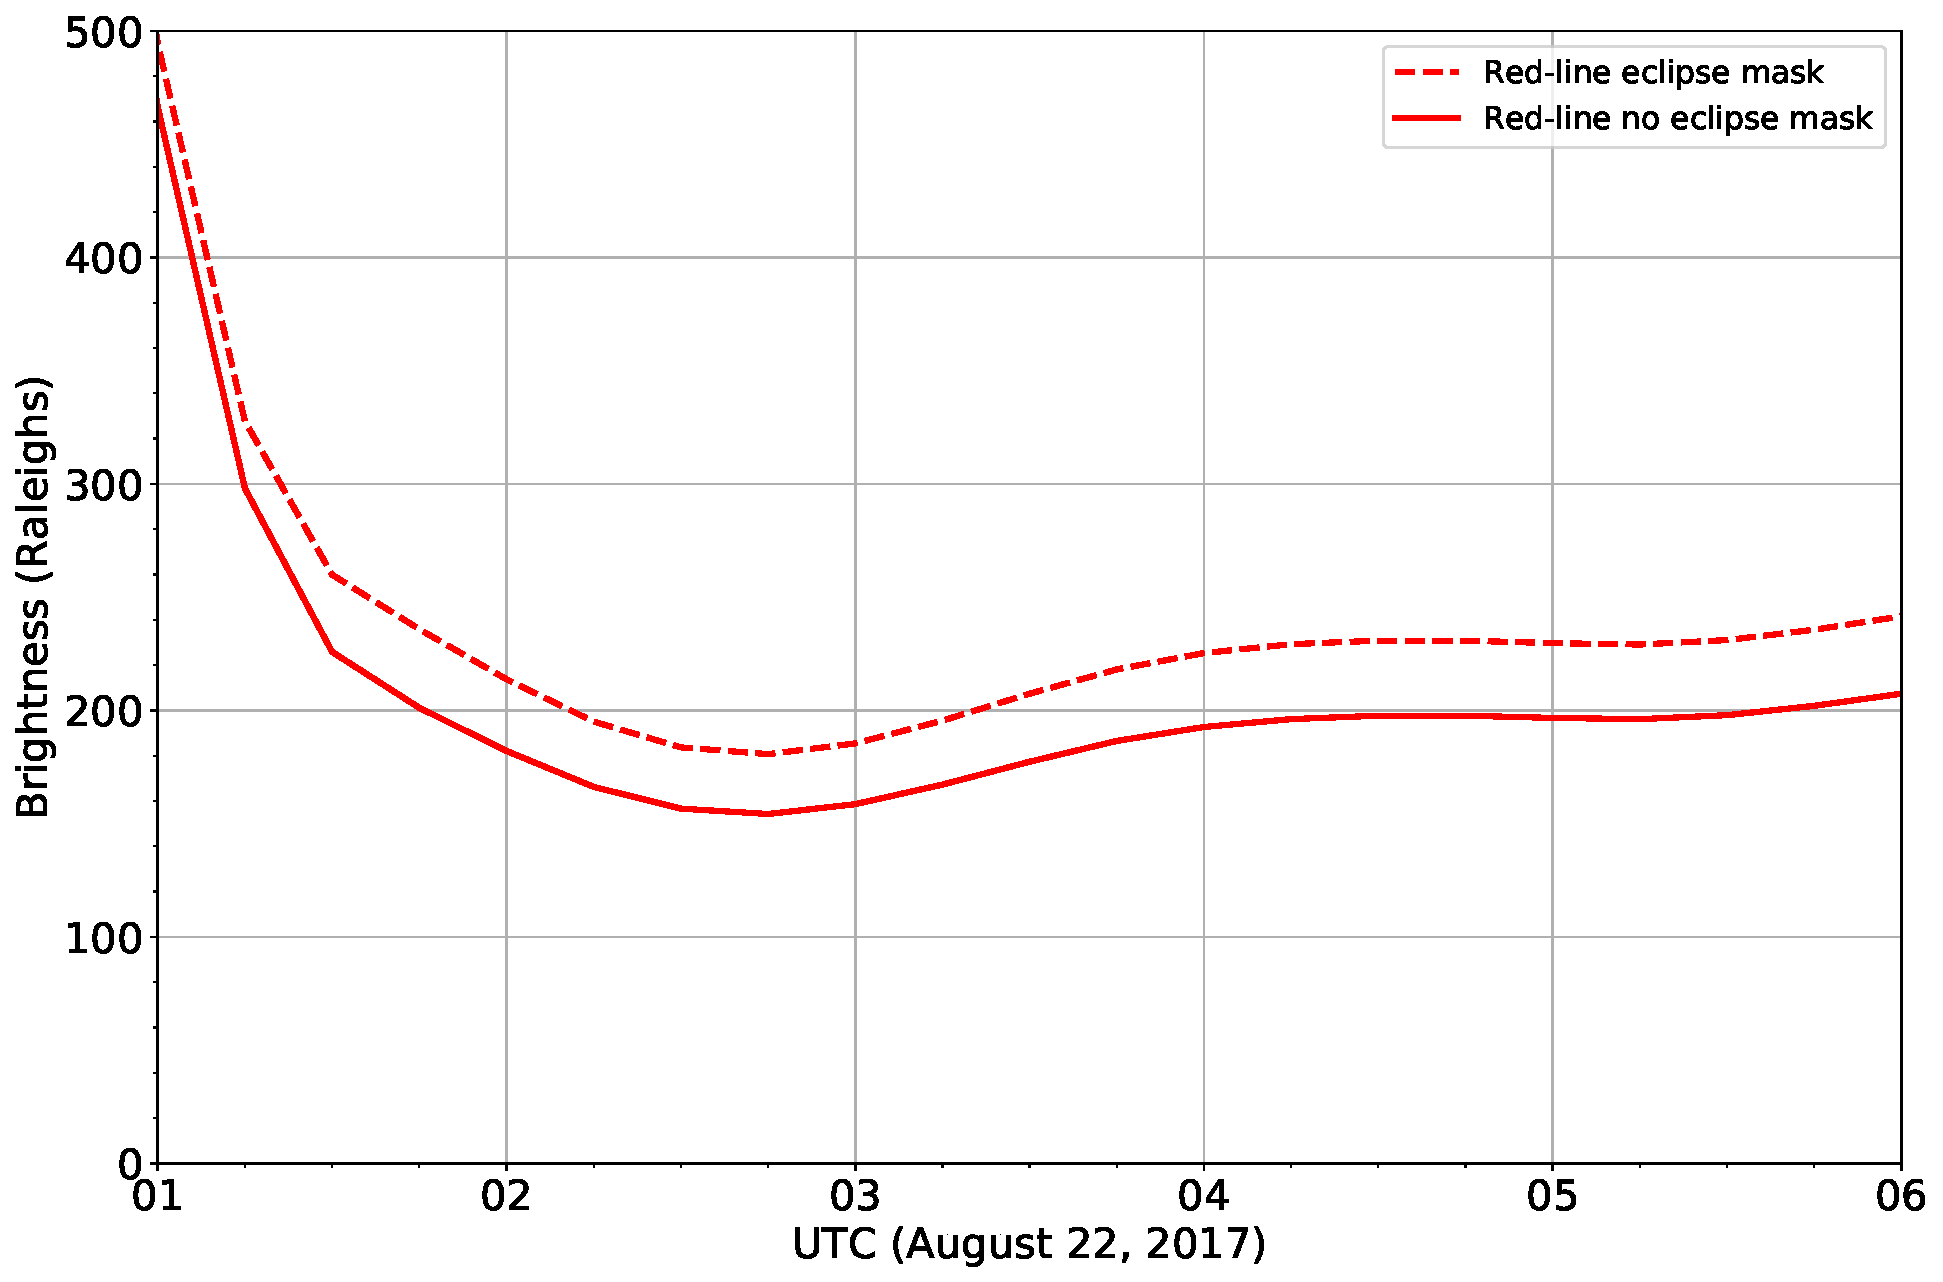
\includegraphics[width=30pc]{GITM_with_GLOW_dglow.pdf}
 \caption{ Red line brightnesses (in arbitrary units) on August 21-22, 2017. Notice around 10\% enhancement on August 22 when compared to August 21.}
 \label{fig:supp}
 \end{figure}
 
Multi-spectral observation from HiT\&MIS would have been sufficient to infer the vertical wave characteristics of the TID; but the brightness perturbation spanned its FOV, so the meridional scale-size of the TID could not have been estimated. Similarly, using the DTEC measurements meridional wave characteristics could have been estimated, but not the vertical wave characteristics. Utilizing multi-instrument observations we were able to characterize the wave properties, and infer that geomagnetic disturbance-induced Joule heating was the most likely source of these TIDs.
% * <icnossen@googlemail.com> 2018-10-09T13:58:57.420Z:
% 
% > predicted geomagnetic disturbance-induced joule heating to be the source as well as characterize the wave properties. 
% This part of the sentence does not work gramatically and I don't think you "predicted" anything. I think you might want to say something like: ", characterize the wave properties, and infer that geomagnetic disturbance-induced Joule heating was the most likely source of these TIDs."
% 
% ^ <temujinparuhang@gmail.com> 2018-10-29T23:29:12.970Z:
% 
% changed as you suggested
%
% ^.
% * <icnossen@googlemail.com> 2018-10-09T13:55:44.893Z:
% 
% > Multi-spectral observation from HiT\&MIS would have been sufficient to infer the vertical wave characteristics of the TID; but the brightness perturbation spanned its FOV, so the scale-size of the TID could not have been estimated.
% I don't understand this. I'm probably confused by what you mean with "scale-size". Does that refer to the horizontal direction?
% 
% ^ <temujinparuhang@gmail.com> 2018-10-29T21:01:02.813Z:
% 
% yes, replaced with "meridional scale size"
%
% ^.
% * <temujinparuhang@gmail.com> 2018-10-04T21:21:06.076Z:
% 
% > Utilizing multi-instrument observations we were able to establish the large-scale nature of the observed TIDs, predicted geomagnetic disturbance induced joule heating to be the source as well as characterize the wave properties. 
% I think we need one more line here to end this section.. open to suggestions
% 
% ^.

% SM: TIDs are becoming a very popular topic. I miss a part where you conclude a narrative into a closed story. At this point, there are observations and a brief discussion. Here you have a place to put the observations into a broader context. What is the contribution of the HIS imager? Are there any know studies of LSTIDs utilizing ground-based imagers of spectrographs? What new contributions do you show with combining 3 remote observation techniques and a model output? What can differences in peak period, and time delay between different observations tell us about the physical processes (you made some comments already there)? etc... 
% * <icnossen@googlemail.com> 2018-09-24T11:35:28.866Z:
% 
% > SM: TIDs are becoming a very popular topic. I miss a part where you conclude a narrative into a closed story. At this point, there are observations and a brief discussion. Here you have a place to put the observations into a broader context. What is the contribution of the HIS imager? Are there any know studies of LSTIDs utilizing ground-based imagers of spectrographs? What new contributions do you show with combining 3 remote observation techniques and a model output? What can differences in peak period, and time delay between different observations tell us about the physical processes (you made some comments already there)? etc... 
% I agree!
% 
% ^ <temujinparuhang@gmail.com> 2018-10-29T21:02:42.450Z.

\section{Summary}
Analysis of wave-like perturbations observed in red and green line brightness from ground-based optical measurements was presented. Additional insight was provided by MUF profiles based on digisonde measurements and GPS-based TEC measurements. Using wavelet analyses, all of the measurements show a similar dominant time period of about 1.5 hours. We conclude that a geomagnetic disturbance starting at midnight UTC on August 22, 2017 enhanced the auroral currents that lead to Joule heating which triggered AGWs and associated LSTIDs propagating towards the equator. Using cross-correlation on the red and the green line brightness profiles, the vertical phase speed was found to be 30~m/s. Similarly, spectral analysis of DTEC keogram was used to estimate the meridional phase speed of 616 m/s. Furthermore, a total solar eclipse had occurred hours earlier over the continental USA (8 hours earlier in Carbondale, IL). By using the GITM simulation, it was seen that preconditioning of the IT system due to eclipse increased N$_e$ and O/N$_2$ ratio at 250~km around 10\% during the observed TID event. However, it is concluded that the eclipse only strengthened the observed TIDs but not cause it.
\end{document}